% Borrador del articulo para Transportation Research Part C (formato Elsevier, elsarticle).
% Compilar en Overleaf (pdfLaTeX + BibTeX). Las tablas y figuras se generan con:
%   python investigacion/articulo/generar_tablas.py
%   python investigacion/articulo/generar_figuras.py
% Los highlights van en un archivo aparte (highlights.txt), como pide la revista.
\documentclass[preprint,12pt,authoryear]{elsarticle}
\usepackage[utf8]{inputenc}
\usepackage{booktabs}
\usepackage{graphicx}
\usepackage{amsmath}
\usepackage[hidelinks]{hyperref}
\usepackage{xcolor}
% placeins: con \FloatBarrier, las tablas y figuras no pasan de seccion
\usepackage{placeins}
% float: [H] fija las tablas de los apendices donde estan en el texto
\usepackage{float}
% adjustbox: una tabla se achica al ancho del texto solo si no cabe; nunca se agranda
\usepackage{adjustbox}
\newcommand{\ajustar}[1]{\adjustbox{max width=\textwidth}{#1}}
% Fracciones: una pagina solo de figuras debe llenarse al 80 por ciento (sin paginas medio vacias)
\renewcommand{\topfraction}{0.9}
\renewcommand{\bottomfraction}{0.8}
\renewcommand{\textfraction}{0.07}
\renewcommand{\floatpagefraction}{0.8}
\newcommand{\todo}[1]{\textcolor{red}{[TODO: #1]}}
\hyphenation{Open-Street-Map}

\journal{Transportation Research Part C}

\begin{document}

\begin{frontmatter}

\title{How much crime data does crime-aware pedestrian routing need? A pre-registered evaluation in cities a model has never seen}

\author{Sergio Alberto Yacolca Cueva\corref{cor1}\fnref{fn1}}
\ead{sayc2104@gmail.com}
\cortext[cor1]{Corresponding author.}
\fntext[fn1]{ORCID: \href{https://orcid.org/0009-0002-0160-5063}{0009-0002-0160-5063}. The author is a student at The Pennsylvania State University. This research was conducted independently, outside any course or research program, without institutional funding, supervision or resources; the views expressed are the author's own.}
\affiliation{organization={Independent researcher},
            city={State College},
            state={Pennsylvania},
            country={USA}}

\begin{abstract}
Crime-aware pedestrian navigation needs street-level crime records that many cities do not publish. We ask how much crime information a city must provide for such routing to avoid future crime. One gradient-boosting risk model per data-availability level (seven levels, from street-level records to none) was trained on four U.S. cities, sealed, and tested in held-out cities whose records stayed encrypted until a pre-registered opening (Philadelphia and Baton Rouge; Tempe in a replacement exam). The routing engine of a working app planned 2,000 random walking trips per city, and each route was scored by the violent crimes recorded on its streets in the following year. With street-level data, lowest-risk routes crossed 28--57\% fewer recorded violent crimes than fastest routes, at a median detour of about one minute (19--45\% over all trips). Coarse categories did about as well as detailed records, and a simple map of past crime about as well as the model. Aggregated data added little to national public data: with zone counts, city-wide totals or public data alone, routes kept about half of the benefit, comparable to a simple rule. In exploratory analyses, both models and simple maps outperformed a published safe-path method whose density kernel spans hundreds of meters, a 2-minute detour limit kept 65--80\% of the reduction, and the router came close to the best feasible route. The main result held with earlier public data, other exclusion rules, and Tempe's misclassified crime categories corrected. For crime-aware routing, the city's data matter more than the predictor.
\end{abstract}

\begin{keyword}
pedestrian navigation \sep safe routing \sep route choice \sep crime risk \sep transfer across cities \sep pre-registration
\end{keyword}

\end{frontmatter}

% =========================================================================
\section{Introduction}

Walking-navigation services usually recommend the fastest route. Pedestrians weigh other attributes of streets as well: route-choice studies based on large samples of smartphone walking trajectories estimate how much extra walking people accept to use streets with the attributes they prefer \citep{sevtsuk2021routechoice,basu2022willingness}. Personal safety is one such concern, although the evidence linking neighborhood crime to walking is mixed \citep{foster2008crime}. Safe-routing systems make the trade-off explicit: they accept a detour in exchange for lower exposure to crime along the route \citep{galbrun2016safe}.

Deploying such a service raises questions that evaluations inside a single data-rich city cannot answer. Safe-routing systems are built on detailed, street-level crime records, and not every city publishes them: some publish only coarse categories, aggregates by district or city-wide totals, and some publish nothing at all. A service operator, or a city deciding which data to release, needs to know:
\begin{enumerate}
  \item whether a risk model trained in cities with good data can be deployed, unchanged, in a new city;
  \item how much of the benefit survives as the city's crime data become scarcer;
  \item how much exposure is avoided for a given detour budget;
  \item whether the recommendations concentrate pedestrians on a few streets;
  \item whether the computation is fast enough for interactive use.
\end{enumerate}

The first two questions are hard to answer credibly. The evaluation must be out-of-city and forward in time: a model that is tuned, even indirectly, on the test city's crimes will look better than it is. It must score the routes that a router would actually recommend, not risk maps in the abstract. And it must report the levels and cities where the approach fails.

This paper reports such an evaluation, organized around one question: how much crime information must a city provide for crime-aware routing to avoid future crime? We contribute:
\begin{enumerate}
  \item \textbf{A data-availability ladder.} Seven levels describe the crime information a city may have, from detailed street-level records to none at all, in three groups: crime by street, aggregated crime, and without crime data. Each level corresponds to a data-release decision a city can make. One model per level is trained on four cities and transferred, unchanged, to new cities.
  \item \textbf{A pre-registered, route-level evaluation.} Cities were assigned to learning, practice and exam groups by lottery. Exam data were downloaded directly into encrypted files, and each encrypted group was opened once, after the models and the evaluation code were fingerprinted and the analysis plan was registered on OSF \citep{osf_main,osf_tempe}. The routes come from the router of a working app and are scored against crimes recorded in the following year. Shuffled-data ``traps'' and an oracle map act as negative and positive controls.
  \item \textbf{An answer: the data matter more than the predictor.} With street-level records, even in broad categories, routes avoided a large share of future recorded violent crime in all three exam cities. A simple map of the city's own past crime did about as well as the transferred model. Aggregated data added little to public data alone: with zone counts, city-wide totals or no crime data, routes kept about half of the benefit, comparable to a simple rule.
  \item \textbf{Transport analyses.} We report, as exploratory analyses, the crime avoided under detour budgets of 2, 5 and 10 minutes, the effect of the recommendations on the concentration of walking across streets, and the time per routing query (Sections~\ref{sec:transport-methods} and~\ref{sec:transport-results}).
  \item \textbf{A comparison with a published method and a stress test.} On the same trips and with the same information, both our models and simple maps of past crime avoided more future violent crime than the safe-path method of \citet{galbrun2016safe}, also in versions of it that use the time of day. In ten further analyses after the exam, specified to address concerns about a draft of this paper, the main result held. One of them uncovered errors in the registered translation of Tempe's crime categories; correcting them left Tempe's route results essentially unchanged.
\end{enumerate}

% =========================================================================
\section{Related work}

\paragraph{Safe routing} \citet{galbrun2016safe} formalized safe paths as a bi-objective problem over a street-level risk map built from crime records in Chicago and Philadelphia; an openly available earlier version describes the same model \citep{galbrun2014safe}. They estimate crime density with a Gaussian kernel whose bandwidth follows Scott's rule \citep{scott1992multivariate}. They define the risk of a path either as the probability of at least one crime along it (total risk) or as the risk of its riskiest segment (maximum risk), and they return the routes on the lower convex hull of length and risk. In the openly available version, the evaluation examined how well this small set of routes represents the trade-off and how fast it is computed. It did not test whether the recommended routes avoided crimes recorded later, nor how the approach transfers to cities with less data.

\paragraph{Pedestrian route choice} Revealed-preference studies using large samples of smartphone walking trajectories estimate how street attributes shape the routes pedestrians take, and express the estimates as willingness to walk or perceived distance \citep{sevtsuk2021routechoice,basu2022willingness}. Such estimates bear on how long a detour a navigation service can reasonably propose. Rather than assume one value, we report the crime avoided under several detour budgets.

\paragraph{Constrained and bi-objective shortest paths} Trading walking time for lower risk is a bi-objective shortest-path problem. Exact methods enumerate all Pareto-optimal paths, while weighted-sum scalarization finds the supported solutions on the convex hull \citep{raith2009biobjective}. Minimizing exposure subject to a limit on the detour is a constrained shortest-path problem, which can be approached by Lagrangian relaxation of the time constraint \citep{handler1980dual}. Our router follows this approach (Section~\ref{sec:routing}).

\paragraph{Crime concentration and environmental risk} Crime concentrates in a small share of street segments in every city studied \citep{weisburd2015law}, which is why avoiding a few streets can matter. Risk terrain modeling predicts risk from environmental features such as bars or transit stops \citep{caplan2011rtm}; our ``no crime data'' level is close in spirit. In long-term forecasts of robbery at micro places, random forests greatly outperformed risk terrain models and kernel density estimates, but only slightly outperformed prior crime counts \citep{wheeler2021rtm}. Our comparisons of models with maps of past crime show a similar pattern (Sections~\ref{sec:results} and~\ref{sec:sensitivity}).

\paragraph{Exposure and the denominator} The apparent danger of a place depends on whether crimes are divided by residents or by the people actually present \citep{andresen2006measures,malleson2015ambient}. We report a secondary per-person metric that divides crimes by simulated pedestrian volumes.

\paragraph{Transfer across cities} Transfer across cities has been used for spatio-temporal prediction in data-scarce cities, demonstrated on crowd flows \citep{wang2019crosscity}. For crime:
\begin{itemize}
  \item knowledge learned in Toronto and Vancouver has been transferred to predict crime in the smaller city of Halifax \citep{bappee2021crossdomain};
  \item unsupervised domain adaptation has been used to predict crime risk in a city without labeled crime data \citep{zhou2023udac};
  \item transfer learning has improved short-term prediction where human-mobility data are scarce \citep{networktransfer2024};
  \item a single model has been trained across cities with different crime categories \citep{hypernetwork2025};
  \item across 12 U.S. cities, transfer generally improved few-shot prediction, but the gains varied with differences between cities and with spatial scale \citep{intercity2026}.
\end{itemize}
These studies predict crime. We evaluate the routes a router would recommend, and we vary the crime information available in the target city systematically, from detailed records to none.

\paragraph{Evaluation and bias} Crime forecasts are commonly evaluated against crimes recorded after the forecast period, including in randomized field trials of predictive policing \citep{mohler2015trials}, and capture-type accuracy measures are common \citep{accuracy2020}. Pre-registration separates confirmatory tests from exploratory analyses \citep{nosek2018prereg}; we label every analysis accordingly. Police records reflect enforcement as well as crime \citep{lum2016predict}; we return to this limitation in Section~\ref{sec:discussion}.

% =========================================================================
\section{Data}\label{sec:data}

\subsection{Cities and groups}
Nine U.S. cities with open, point-level police incident data were divided into groups before any model development, using a reproducible lottery (Python \texttt{random}, seed chosen by the author, 4818):
\begin{itemize}
  \item \textbf{Learning:} Pittsburgh (fixed, because its data had already been seen), Chapel Hill, Chicago and Seattle.
  \item \textbf{Practice:} Cincinnati and Gainesville. These were used to compare four model iterations, all logged.
  \item \textbf{Main exam:} one large, one medium and one university city, each drawn within its stratum: Philadelphia, Baton Rouge and Tempe.
\end{itemize}
Eight further cities are kept closed for a future version: four in an external reserve and four set aside for an additional check at the zone level.

\subsection{Outcome and periods}
The outcome is the \emph{universal core}: the FBI's violent crimes without rape, namely murder and non-negligent manslaughter (NIBRS 09A), robbery (120) and aggravated assault (13A) \citep{fbi2023nibrs}. Every incident counts as one; an incident with an unknown hour is split equally across the four time bands. Rape is excluded in every city because some cities hide its location. Each city's categories were translated into these codes with tables written before its data were opened, from official documentation only: UCR codes for Philadelphia, NIBRS codes for Baton Rouge and keyword rules for Tempe. Tempe's rules misclassified part of its records; a post-exam audit and its effect are reported in Section~\ref{sec:sensitivity}.

Periods are identical for every city: the \emph{past} (1 January 2024 to 31 August 2025) may be used to build a city's map; the \emph{future} (1 September 2025 to 31 August 2026) is scored. Incidents were excluded if they had no valid date or location, were sexual offenses, fell outside the city boundary, lay more than 50 m from a walkable street, or lay less than 30 m from a prison, hospital, police station or social facility. Table~\ref{tab:datos} summarizes the exam data, and Table~\ref{tab:exclusiones} in \ref{app:modelo} gives the exclusions by reason.

\begin{table}[htbp]
\centering\small
\caption{Exam data. ``Core incidents kept'' are violent crimes (09A, 120, 13A) in both periods after exclusions. Months covered: share of the 32 study months with at least one record.}
\label{tab:datos}
\ajustar{\begin{tabular}{lrrrrr}
\toprule
City & Records read & In study period & Kept after exclusions & Core incidents kept & Months covered \\
\midrule
Philadelphia & 596,971 & 413,305 & 382,054 & 29,799 & 100\% \\
Baton Rouge & 147,177 & 67,021 & 54,379 & 4,282 & 100\% \\
Tempe & 384,814 & 76,143 & 68,679 & 1,736 & 100\% \\
\bottomrule
\end{tabular}
}
\end{table}

\subsection{Public features}
Every level except Map only uses the following nationally available public data; Map only uses the OpenStreetMap features alone:
\begin{itemize}
  \item street-network form and places from OpenStreetMap, read from Geofabrik extracts \citep{osm_geofabrik} with the walkable-network filter of OSMnx \citep{boeing2017osmnx};
  \item 2020 Census population \citep{census2020blocks} and 2023 LEHD jobs \citep{lodes8}, by Census block;
  \item GTFS transit schedules of each city's main operator \citep{mobilitydatabase};
  \item VIIRS night-time radiance, the median of 30 nights up to 31 August 2025 \citep{nasa_gibs_viirs};
  \item simulated pedestrian volumes by time band.
\end{itemize}
The simulated volumes come from a trip-based gravity model built only from the data above (\ref{app:peatones}). In an out-of-sample test against pedestrian counts at 98 locations in New York City, the variant used here, which takes transit activity from schedules, ranked locations with a Spearman correlation of 0.56. With observed transit ridership, the correlation was 0.67. A standard direct-demand regression fitted to local counts did better (0.81), but it requires counts that most cities lack.

No race, ethnicity, income or poverty-proxy variable is used, and no feature identifies a place: no coordinates, no street names, no city identity.

% =========================================================================
\section{Methods}\label{sec:methods}

\subsection{Data-availability levels}
Table~\ref{tab:niveles} lists the levels in three groups. The letters in parentheses are the codes used in the registrations. Core only (A) and Coarse (C) are alternatives rather than steps: fewer but exactly classified incidents, against all incidents in coarse bags. All levels may use what was learned in the learning cities; they differ in which \emph{past} crime information of the evaluated city enters the model. Crime features are spread to nearby streets: weight 1 up to a walking distance of 40 m, decreasing by 10 percentage points every 20 m, and zero beyond 220 m. They are then expressed relative to the city mean in each time band, so that cities with different crime levels are comparable. In the exam cities, every level is obtained by withholding information that these cities do publish. A city that truly publishes less may also differ in other ways, for example in how it records crime.

\begin{table}[htbp]
\centering\small
\caption{Data-availability levels.}
\label{tab:niveles}
\begin{tabular}{llp{0.45\textwidth}}
\toprule
Group & Level (code) & Past crime information of the evaluated city \\
\midrule
Crime by street & Detailed (B) & All incidents by street, with ten broad categories \\
 & Core only (A) & Core violent incidents by street \\
 & Coarse (C) & All incidents by street, in three bags (violent / property / other) \\
\midrule
Aggregated crime & Zone & Core incidents per Census block group \\
 & City total & City-wide core rate per 1,000 residents \\
\midrule
Without crime data & No crime data & None \\
 & Map only & None, and only OpenStreetMap features \\
\bottomrule
\end{tabular}
\end{table}

\subsection{Model}
For each level, one LightGBM model \citep{ke2017lightgbm} is trained on the learning cities. Each training row is a street segment and time band. The target is the segment's future core risk (future incidents spread as above), and the inputs are the segment's public features and the past crime features its level allows. The settings are:
\begin{itemize}
  \item Tweedie loss with variance power 1.5;
  \item 400 rounds, learning rate 0.05, 31 leaves, at least 200 rows per leaf;
  \item feature and bagging fractions of 0.8, bagging at every round, L2 regularization of 1 and random seed 7;
  \item segment type and time band as categorical features;
  \item each learning city weighted equally.
\end{itemize}
\ref{app:modelo} lists every feature of every level. Four iterations, labeled v0, v0.1, v1 and v2 in the practice log, were compared on the practice cities; the last (v2) was sealed and is the only one evaluated here. The learning cities use the same past and future periods as the exam cities. The models were therefore trained on outcomes from the same period in which they were evaluated (September 2025 to August 2026), although in other cities; a deployed system would train on an earlier period.

\subsection{Routing}\label{sec:routing}
Routes come from the router of a working safe-routing app, with its search unchanged. The router addresses the constrained problem of minimizing predicted exposure subject to a limit on the extra walking time, by Lagrangian relaxation of the time constraint \citep{handler1980dual}:
\begin{itemize}
  \item For each trip it computes the fastest route and the routes that minimize walking time plus $\lambda$ times the predicted exposure along the route, for $\lambda \in \{0.5, 1, 2, 4, 8, 16\}$.
  \item It then refines $\lambda$ by five bisection steps, on a logarithmic scale, between the largest value whose route respects the time limit and the smallest value whose route does not.
  \item It also generates up to three spatially distinct alternatives by penalizing streets already used. These are kept only if their predicted exposure is not more than 3\% above the fastest route's.
\end{itemize}
The exposure of a segment is its length times the sum of its predicted risk per meter and a background term equal to three times the city's mean risk; the background term discourages long detours. A route is discarded if its extra walking time exceeds the larger of 10 minutes and half the fastest route's walking time. Among the remaining routes, the one with the lowest predicted exposure is offered as the ``lowest-risk'' route if its predicted exposure is at least 3\% lower than the fastest route's, and if the predicted risk alone, without the background term, is also lower. Walking speed is 80 m/min, and no waiting time is added at crossings. Two features of the app were not used in the exam. The first is a night-time penalty for unlit streets (predicted risk multiplied by 1.27 in the two night bands), which the app applies on top of the risk map. The second is the calibration of the percentage shown to users, which does not change which route is offered.

\subsection{Evaluation}
\paragraph{Trips} In each city, 2,000 walking trips are drawn at random: the origin is a node of the walking network, and the destination a node 500--3,000 m away in a straight line. Trips cycle through four hours (2 a.m., 9 a.m., 3 p.m. and 9 p.m.), one in each of the model's time bands (midnight to 6 a.m., 6 a.m. to noon, noon to 6 p.m. and 6 p.m. to midnight), and the seed is fixed per city. Every map is applied to the same trips.

\paragraph{Primary metric} The route change is the total number of future core incidents on the street segments of the lowest-risk routes, divided by the same total on the fastest routes, minus one, over the trips where the router offers a lowest-risk route. Only incidents in the trip's time band are counted. Segments shared by both routes count on both sides. The 95\% confidence interval comes from 2,000 bootstrap resamples of trips. Because each map offers an alternative on a different set of trips, we also report, as an exploratory measure, the change \emph{over all trips}, which has a common denominator: each trip takes the lowest-risk route when one is offered and the fastest route otherwise.

\paragraph{Secondary metrics}
\begin{itemize}
  \item \textbf{Per-person change:} the route change after dividing each segment's incidents by its simulated pedestrians.
  \item \textbf{Extra minutes:} the median extra walking time of the lowest-risk route.
  \item \textbf{Retention:} the route change of a level divided by that of Detailed (B), computed on the trips where both maps offered a lowest-risk route. It therefore cannot be obtained by dividing entries of Table~\ref{tab:rutas}, which use each map's own trips.
  \item \textbf{Quick capture:} the share of future core incidents in the 10\% of network length that the map ranks as riskiest; its interval comes from resampling 1-km zones (results in \ref{app:rapida}).
\end{itemize}

\paragraph{Comparators} None of these is a trained model:
\begin{itemize}
  \item \textbf{heat maps A and B:} the evaluated city's past crimes, spread as above, with the information of Core only (A) and of Detailed (B);
  \item \textbf{``avoid arterials'':} risk rises near main roads;
  \item \textbf{``avoid commercial areas'':} risk rises with the number of shops and selected amenities within 400 m, the same count the models use as a feature;
  \item \textbf{an oracle:} the future crimes themselves, spread. It is an impossible ceiling.
\end{itemize}

\subsection{Pre-registration and safeguards}
\paragraph{The vault} Exam data were downloaded directly into files encrypted with AES-256-GCM, with no plaintext copy on disk: on 3 October 2026 for the main exam and on 8 October 2026 for Tempe's replacement exam (Section~\ref{sec:deviations}). The passphrase is known only to the author and was never given to the AI system used to help write code. Every development script loaded a guard that stopped it if it tried to open the vault files; only the vault program, with the passphrase, could decrypt them. The strong protection was the encryption itself.

\paragraph{The seal} Before opening, the model files and the evaluation code were fingerprinted (SHA-256) and tagged in version control, and the plan was registered \citep{osf_main}.

\paragraph{The opening} The exam program refuses to run if any model fingerprint differs from the seal. Before computing any result, it checks only that the files could be read.

\paragraph{The controls}
\begin{itemize}
  \item \textbf{Two negative controls (``traps''):} the best map with its values shuffled among street segments within each time band, and the real map scored against future crimes shuffled in the same way. Each must score near chance; otherwise the city's exam is invalid. The registered rules are:
  \begin{itemize}
    \item \emph{quick capture:} a trap's capture must not exceed the midpoint between the chance level and the real map's capture. If the real map's lower 95\% bound does not exceed chance, the trap's lower bound must not exceed chance instead (rule clarified before the Tempe exam; Section~\ref{sec:deviations});
    \item \emph{routes:} when the real map reduces crime, the shuffled map must avoid less than half as much future crime as the real map; otherwise it must show no clear reduction (upper 95\% bound at or above zero).
  \end{itemize}
  \item \textbf{One positive control:} the oracle must reduce crime; otherwise the pipeline is investigated before interpretation.
\end{itemize}

\paragraph{Hypotheses} Each hypothesis had to hold in all three cities.
\begin{itemize}
  \item \textbf{H1:} the three crime-by-street levels, Detailed (B), Core only (A) and Coarse (C), reduce future core crime (upper bound of the 95\% CI below 0\%).
  \item \textbf{H2:} the Core-only (A) and Detailed (B) models are non-inferior to the heat map of the same data (upper bound of the paired difference below $+5$ percentage points), or superior (below 0).
  \item \textbf{H3a:} the No-crime-data level reduces future core crime.
  \item \textbf{H3b:} the No-crime-data level beats each simple rule.
\end{itemize}
The paired differences of H2 and H3b are computed on the trips where both maps offered a lowest-risk route, with intervals from resampling those trips.

\subsection{Transport analyses (exploratory)}\label{sec:transport-methods}
After the exams, we specified three further analyses and committed the plan to version control before writing their code. They use the exam data already opened and the risk maps already computed; no model or registered result was changed.
\begin{enumerate}
  \item \textbf{Detour budget.} The router was rerun with the limit on extra walking time fixed at 2, 5 and 10 minutes instead of the app's default limit (the larger of 10 minutes and half the fastest route's walking time). Everything else in the router was unchanged. This was done for three maps (Detailed (B), No crime data and the oracle) on the same 2,000 trips per city. The outcome is the change over all trips: each trip takes the lowest-risk route if one is offered and the fastest route otherwise. Its 95\% interval comes from 2,000 resamples of 1-km origin zones. We also report the share of trips with an alternative and, over those trips, the median extra walking time.
  \item \textbf{Concentration of walking.} If every trip followed the app's suggestion, would walking concentrate on fewer streets? On the exam trips (default limit), for Detailed (B) and No crime data, we compare the suggested routes with the fastest routes by three measures: the number of distinct segments used, the share of walked meters on the 1\% most-used segments, and the Gini index of walked meters per segment. The trips are a random sample, not observed demand, so this analysis is descriptive.
  \item \textbf{Computation.} We timed each routing query, excluding the loading of the network, for the first 200 trips of each city with the Detailed (B) map, in a single process. We report the median and the 95th percentile, together with the hardware used.
\end{enumerate}

% =========================================================================
\section{Results}\label{sec:results}
This section reports the registered analyses; Section~\ref{sec:exploratory} reports the exploratory ones.

\subsection{Controls}
In all three cities the oracle removed most future violent crime from the routes, and every trap scored at chance level (Table~\ref{tab:controles}). Shuffled maps captured 0.07--0.11 of future crime, against a chance level of 0.10; the real Detailed (B) maps captured 0.43--0.58. The routes chosen with shuffled maps changed crime by $+2\%$ to $+11\%$. There is no sign of information leaking from the exam data into the models.

\begin{table}[htbp]
\centering\small
\caption{Positive control (oracle) and negative controls (traps). Capture = share of future core incidents in the riskiest 10\% of network length (chance level in each pair). Route changes in \%.}
\label{tab:controles}
\ajustar{\begin{tabular}{lcccccc}
\toprule
 & \begin{tabular}[b]{@{}c@{}}Oracle: route \\ change, \% (95\% CI)\end{tabular} & \begin{tabular}[b]{@{}c@{}}Shuffled map: \\ capture / chance\end{tabular} & \begin{tabular}[b]{@{}c@{}}Shuffled future: \\ capture / chance\end{tabular} & \begin{tabular}[b]{@{}c@{}}Real map: \\ capture\end{tabular} & \begin{tabular}[b]{@{}c@{}}Shuffled map: \\ route change, \%\end{tabular} & Traps \\
\midrule
Philadelphia & -83 (-85, -80) & 0.101 / 0.100 & 0.120 / 0.124 & 0.426 & +2 & all pass \\
Baton Rouge & -91 (-94, -87) & 0.109 / 0.100 & 0.129 / 0.145 & 0.467 & +11 & all pass \\
Tempe & -92 (-95, -89) & 0.074 / 0.100 & 0.121 / 0.158 & 0.575 & +3 & all pass \\
\bottomrule
\end{tabular}
}
\end{table}

\subsection{Route outcomes by data level}
Figure~\ref{fig:escalera} summarizes the main result by data level and city, and Table~\ref{tab:rutas} gives the route change of every map, including the comparators.

\begin{figure}[htbp]
\centering
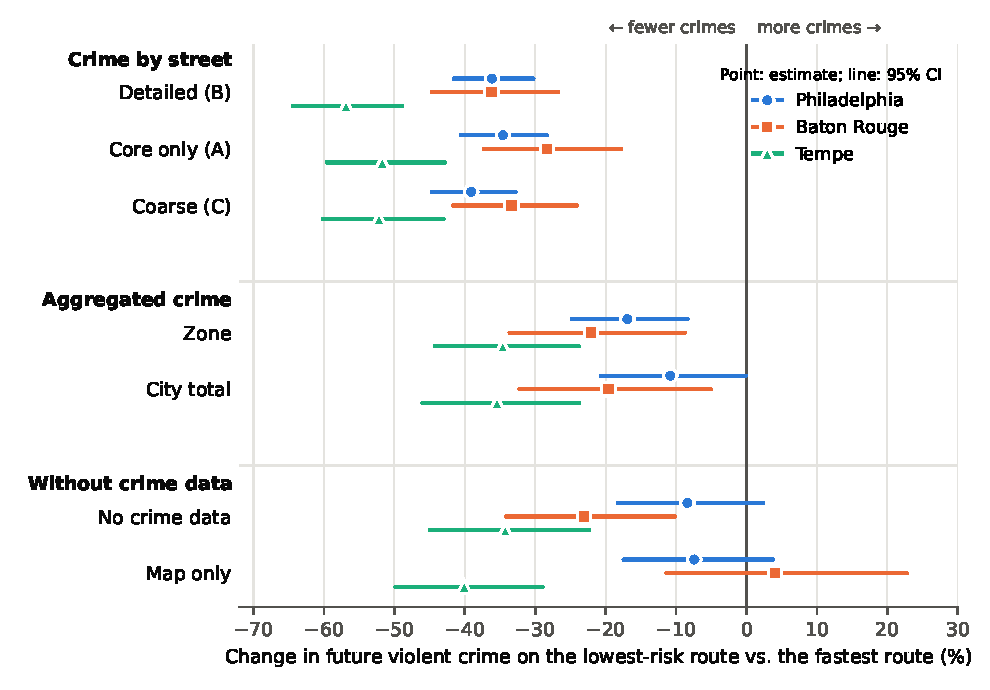
\includegraphics[width=\textwidth]{figuras/fig_escalera.pdf}
\caption{Change in future violent crime (murder, robbery, aggravated assault; September 2025 to August 2026) on the lowest-risk route compared with the fastest route, by data-availability level, in three cities the models never saw. Points are estimates and lines 95\% bootstrap intervals, over trips where the router offered a lowest-risk route. Values left of zero mean fewer crimes. The numbers are in Table~\ref{tab:rutas}.}
\label{fig:escalera}
\end{figure}

\begin{itemize}
  \item \textbf{With street-level crime data,} lowest-risk routes crossed 35--39\% fewer future violent crimes than fastest routes in Philadelphia, 28--36\% fewer in Baton Rouge and 52--57\% fewer in Tempe. The median extra walking time was 0.6--1.3 minutes.
  \item \textbf{Retention:} Coarse (C) retained 0.95--1.06 of the benefit of Detailed (B), with 95\% intervals from 0.81 to 1.18, and Core only (A) 0.77--1.00 (Table~\ref{tab:retencion}). These intervals are compatible with equal performance, but formal equivalence was not registered and is not claimed.
  \item \textbf{With less information, the benefit fell, and aggregated data added little to public data alone.} The aggregated levels, Zone and City total, retained 0.45--0.64 of the benefit, and No crime data 0.44--0.59. City total changed future crime on routes by $-11\%$, $-20\%$ and $-35\%$ in the three cities, close to No crime data ($-8\%$, $-23\%$ and $-34\%$) and to the ``avoid commercial areas'' rule ($-12\%$, $-20\%$ and $-29\%$); Zone did slightly better in Philadelphia ($-17\%$). Without crime data, the interval in Philadelphia included zero (95\% CI $-18$ to $+2$). Map only, which uses OpenStreetMap features alone, varied the most: $-7\%$ in Philadelphia, no effect in Baton Rouge ($+4\%$, 95\% CI $-11$ to $+23$; retention 0.01) and $-40\%$ in Tempe.
  \item \textbf{The simple rules behaved very differently across cities.} ``Avoid arterials'' \emph{increased} crime on routes in Philadelphia ($+11\%$; $+13\%$ in Baton Rouge, with an interval that included zero), but in Tempe ($-37\%$) it did about as well as the No-crime-data model ($-34\%$).
\end{itemize}

\begin{table}[htbp]
\centering\small
\caption{Change in future core incidents on lowest-risk vs.\ fastest routes, \% (95\% CI), over trips where the router offered a lowest-risk route (38--67\% of trips for the crime-by-street levels).}
\label{tab:rutas}
\begin{tabular}{lccc}
\toprule
Map & Philadelphia & Baton Rouge & Tempe \\
\midrule
Detailed (B) & -36 (-42, -30) & -36 (-45, -27) & -57 (-64, -49) \\
Core only (A) & -35 (-41, -28) & -28 (-37, -18) & -52 (-60, -43) \\
Coarse (C) & -39 (-45, -33) & -33 (-42, -24) & -52 (-60, -43) \\
\midrule
Zone & -17 (-25, -8) & -22 (-34, -9) & -35 (-44, -24) \\
City total & -11 (-21, -0.1) & -20 (-32, -5) & -35 (-46, -24) \\
\midrule
No crime data & -8 (-18, +2) & -23 (-34, -10) & -34 (-45, -22) \\
Map only & -7 (-17, +4) & +4 (-11, +23) & -40 (-50, -29) \\
\midrule
Heat map B (no model) & -34 (-40, -29) & -28 (-36, -19) & -54 (-61, -46) \\
Heat map A (no model) & -27 (-33, -21) & -20 (-29, -9) & -31 (-40, -22) \\
Rule: avoid commercial areas & -12 (-23, -1) & -20 (-38, +0) & -29 (-42, -13) \\
Rule: avoid arterials & +11 (+1, +23) & +13 (-4, +33) & -37 (-48, -25) \\
\midrule
Oracle (future crime; ceiling) & -83 (-85, -80) & -91 (-94, -87) & -92 (-95, -89) \\
\bottomrule
\end{tabular}

\end{table}

\begin{table}[htbp]
\centering\small
\caption{Retention of the Detailed (B) benefit: route change of each level divided by that of Detailed (B), on the same trips (95\% CI).}
\label{tab:retencion}
\begin{tabular}{lccc}
\toprule
Level & Philadelphia & Baton Rouge & Tempe \\
\midrule
Core only (A) & 1.00 (0.89, 1.12) & 0.77 (0.58, 0.95) & 0.90 (0.78, 1.02) \\
Coarse (C) & 1.06 (0.95, 1.18) & 0.95 (0.81, 1.10) & 1.01 (0.90, 1.11) \\
\midrule
Zone & 0.53 (0.32, 0.71) & 0.54 (0.26, 0.77) & 0.62 (0.45, 0.77) \\
City total & 0.50 (0.19, 0.75) & 0.45 (0.14, 0.72) & 0.64 (0.46, 0.80) \\
\midrule
No crime data & 0.44 (0.12, 0.69) & 0.59 (0.28, 0.86) & 0.59 (0.40, 0.75) \\
Map only & 0.36 (0.01, 0.62) & 0.01 (-0.60, 0.41) & 0.66 (0.51, 0.82) \\
\bottomrule
\end{tabular}

\end{table}

\subsection{Pre-registered hypotheses}
Table~\ref{tab:hipotesis} applies the registered decision rules.
\begin{itemize}
  \item \textbf{H1 held for the three crime-by-street levels in all three cities.}
  \item \textbf{H2 (Core only, A):} non-inferior to its heat map in all three cities and superior in two.
  \item \textbf{H2 (Detailed, B):} non-inferior in Philadelphia and superior in Baton Rouge. In Tempe the paired difference was $-0.3$ percentage points, but the upper bound of its interval ($+5.09$) exceeded the $+5$ margin by 0.09, so non-inferiority was not shown.
  \item \textbf{H3a and H3b} were not supported across the three cities.
  \item \textbf{Superiority was clear only for Core only (A) in Tempe.} The upper bounds of the paired differences were $-7.9$ points there, but only $-1.6$ for Core only (A) and $-2.2$ for Detailed (B) in Baton Rouge, close to zero. Over all trips, an exploratory measure, the model and the heat map of the same detailed data did not differ clearly in any city, and with core crime only the model was clearly better only in Tempe (Section~\ref{sec:sensitivity}).
\end{itemize}

\begin{table}[htbp]
\centering\small
\caption{Pre-registered hypotheses. Cells give the verdict and, in parentheses, the upper bound of the relevant 95\% CI: the route change in \% (H1, H3a) or the paired difference in percentage points (H2, H3b; non-inferiority margin $+5$). Philadelphia and Baton Rouge come from the main exam; Tempe from the replacement exam (Section~\ref{sec:deviations}).}
\label{tab:hipotesis}
\ajustar{\begin{tabular}{lcccc}
\toprule
Hypothesis & Philadelphia & Baton Rouge & Tempe & All three \\
\midrule
H1: Detailed (B) reduces crime & yes (-30) & yes (-27) & yes (-49) & yes \\
H1: Core only (A) reduces crime & yes (-28) & yes (-18) & yes (-43) & yes \\
H1: Coarse (C) reduces crime & yes (-33) & yes (-24) & yes (-43) & yes \\
H3a: No crime data reduces crime & no (+2) & yes (-10) & yes (-22) & no \\
H2: Core only (A) vs.\ heat map A & non-inferior (+3.0) & superior (-1.6) & superior (-7.9) & non-inferior \\
H2: Detailed (B) vs.\ heat map B & non-inferior (+4.4) & superior (-2.2) & no (+5.1) & no \\
H3b: no crime data vs.\ avoid arterials & superior (-6.2) & superior (-12.3) & no (+14.2) & no \\
H3b: no crime data vs.\ avoid commercial & no (+8.6) & no (+9.1) & no (+8.3) & no \\
\bottomrule
\end{tabular}
}
\end{table}

\subsection{Per-person change}
The registered secondary metric divides each segment's future crimes by its simulated pedestrians, so it approximates risk per person passing rather than total exposure (Table~\ref{tab:porpersona}).
\begin{itemize}
  \item \textbf{Crime by street.} The per-person change was negative in every city: $-10\%$ to $-13\%$ in Philadelphia, $-21\%$ to $-29\%$ in Baton Rouge and $-16\%$ to $-28\%$ in Tempe. The intervals are wide; they exclude zero for Detailed (B) in Baton Rouge and Tempe and for Core only (A) in Tempe.
  \item \textbf{Aggregated or no crime data.} Results diverged. In Philadelphia, the City total and No-crime-data levels \emph{increased} per-person risk ($+40\%$ and $+47\%$): routes avoided crowded streets with many recorded crimes but used emptier ones. In Baton Rouge the same levels reduced it ($-39\%$ and $-31\%$).
\end{itemize}
Reducing total exposure is therefore not the same as reducing each walker's risk, especially when the model has no crime data. The per-person metric depends on simulated volumes and, as Section~\ref{sec:sensitivity} shows, on the floor applied to sparsely walked segments, so it should be read as indicative only.

\begin{table}[htbp]
\centering\small
\caption{Per-person change (registered secondary metric): change in future core incidents per simulated pedestrian on lowest-risk vs.\ fastest routes, \% (95\% CI), over trips with a lowest-risk route. Each segment's incidents are divided by its simulated pedestrians in that time band, with a floor at the median of segments with pedestrians.}
\label{tab:porpersona}
\ajustar{\begin{tabular}{lccc}
\toprule
Map & Philadelphia & Baton Rouge & Tempe \\
\midrule
Detailed (B) & -13 (-26, +1) & -29 (-46, -8) & -27 (-49, -0.3) \\
Core only (A) & -10 (-23, +3) & -21 (-40, +4) & -28 (-49, -2) \\
Coarse (C) & -10 (-23, +7) & -27 (-49, +3) & -16 (-43, +18) \\
\midrule
Zone & +9 (-7, +28) & -13 (-32, +12) & -17 (-39, +9) \\
City total & +40 (+17, +67) & -39 (-54, -18) & -14 (-38, +16) \\
\midrule
No crime data & +47 (+23, +72) & -31 (-49, -9) & -6 (-32, +29) \\
Map only & +11 (-10, +40) & +7 (-20, +46) & -31 (-51, -5) \\
\midrule
Heat map B (no model) & -17 (-29, -4) & -4 (-26, +26) & -23 (-44, +4) \\
Heat map A (no model) & +5 (-7, +19) & +6 (-20, +38) & -16 (-38, +11) \\
Rule: avoid commercial areas & +8 (-16, +38) & -16 (-55, +46) & +1 (-40, +63) \\
Rule: avoid arterials & +12 (-8, +36) & +25 (-13, +85) & -6 (-36, +39) \\
\midrule
Oracle (future crime; ceiling) & -83 (-86, -79) & -88 (-95, -80) & -88 (-97, -77) \\
\bottomrule
\end{tabular}
}
\end{table}

% =========================================================================
\section{Exploratory analyses}\label{sec:exploratory}
The analyses in this section were run after the exam data had been opened, so they are exploratory: they examine the registered result but do not replace it. Except for the robustness checks of Section~\ref{sec:robustness}, each was specified in a plan committed to version control before its code was written, and the plans are openly available (see Data and code availability). Tables not shown in the text are in \ref{app:sensibilidad}.

\subsection{Robustness of the registered measure}\label{sec:robustness}
Three checks were run after the results were known (\ref{app:sensibilidad}, Table~\ref{tab:robustez}).
\begin{enumerate}
  \item \textbf{Spatial clustering.} Trips may share streets, so we resampled 1-km and 2-km zones of trip origins instead of trips. The intervals barely changed: the median street segment was used by a single trip.
  \item \textbf{Randomness of crime counts.} We also redrew each future count from a Poisson distribution, with the same draw shared by every trip through that segment. This asks whether the effect would persist with another, similar year of crime. Under this stricter interval, the three crime-by-street levels remained below zero in all three cities. The No-crime-data level remained below zero only in Tempe.
  \item \textbf{All trips.} When every trip takes the lowest-risk route if one is offered and the fastest otherwise, future violent crime on routes fell by 23--27\% in Philadelphia, 19--26\% in Baton Rouge and 41--45\% in Tempe (crime-by-street levels).
\end{enumerate}

\subsection{Detour budget, concentration of walking and computation}\label{sec:transport-results}

\paragraph{Detour budget} Figure~\ref{fig:curva} and Table~\ref{tab:curva} show how the change in future violent crime over all trips varies with the limit on extra walking time. Table~\ref{tab:curvacosto} in \ref{app:sensibilidad} gives the share of trips with an alternative and the median extra minutes.
\begin{itemize}
  \item \textbf{Most of the benefit came from short detours.} With Detailed (B) and a 2-minute limit, future violent crime on routes fell by 17--35\% over all trips, against 25--45\% with the app's default limit. The ratio of these point estimates was 0.65--0.80 at 2 minutes and 0.87--0.96 at 5 minutes. The median extra walking time of the trips with an alternative was 0.4--0.5 minutes at the 2-minute limit and 0.6--1.1 minutes at the default limit. All intervals excluded zero at every limit.
  \item \textbf{Without crime data, a larger budget did not help.} The change stayed between $-2\%$ and $-3\%$ in Philadelphia (with intervals that included zero at every limit), between $-9\%$ and $-12\%$ in Baton Rouge and between $-21\%$ and $-22\%$ in Tempe. What limited the benefit was the map, not the detour.
  \item \textbf{With the oracle, the budget mattered more.} Its reduction grew from 54--71\% at 2 minutes to 75--89\% at the default limit. With the Detailed (B) map, the gains beyond 5 minutes were small.
\end{itemize}

\begin{figure}[htbp]
\centering
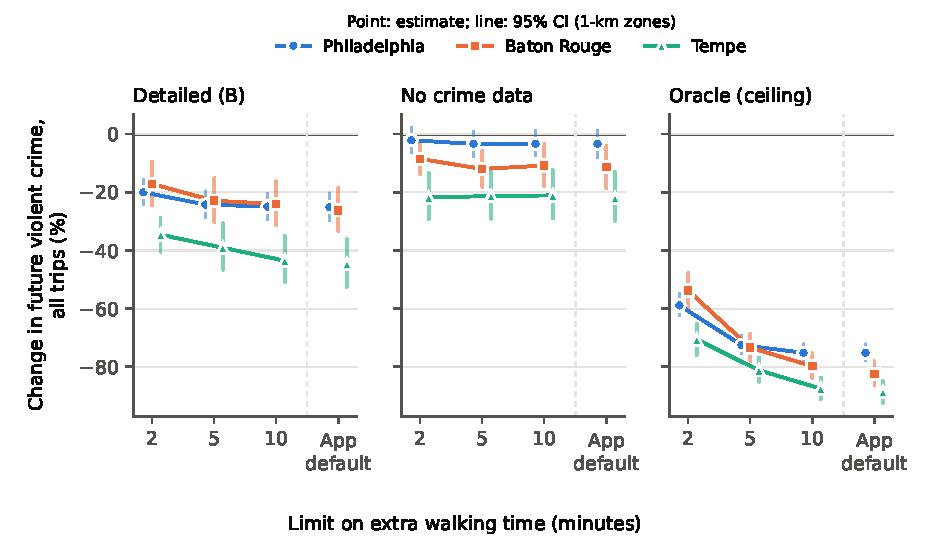
\includegraphics[width=\textwidth]{figuras/fig_curva.pdf}
\caption{Detour budget (exploratory). Change in future violent crime over all trips (lowest-risk route when offered, otherwise the fastest) as the limit on extra walking time varies, for the Detailed (B) map, the No-crime-data map and the oracle. The app's default limit is the larger of 10 minutes and half the fastest route's walking time. Points are estimates and lines 95\% intervals from resampling 1-km origin zones; same 2,000 trips per city. The numbers are in Table~\ref{tab:curva}.}
\label{fig:curva}
\end{figure}

\begin{table}[htbp]
\centering\small
\caption{Detour budget (exploratory): change in future core incidents over all trips (lowest-risk route when offered, otherwise the fastest), \% (95\% CI resampling 1-km origin zones).}
\label{tab:curva}
\begin{tabular}{llccc}
\toprule
Map & Detour limit & Philadelphia & Baton Rouge & Tempe \\
\midrule
Detailed (B) & 2 min & -20 (-24, -16) & -17 (-25, -9) & -35 (-41, -29) \\
 & 5 min & -24 (-29, -20) & -23 (-30, -15) & -39 (-47, -31) \\
 & 10 min & -25 (-29, -20) & -24 (-31, -16) & -44 (-51, -35) \\
 & App default & -25 (-30, -20) & -26 (-33, -18) & -45 (-53, -36) \\
\midrule
No crime data & 2 min & -2 (-6, +2) & -9 (-14, -3) & -22 (-29, -13) \\
 & 5 min & -3 (-8, +1) & -12 (-18, -6) & -21 (-29, -12) \\
 & 10 min & -3 (-7, +1) & -11 (-18, -3) & -21 (-29, -12) \\
 & App default & -3 (-8, +1) & -11 (-19, -4) & -22 (-30, -13) \\
\midrule
Oracle (ceiling) & 2 min & -59 (-62, -55) & -54 (-60, -48) & -71 (-76, -65) \\
 & 5 min & -73 (-75, -69) & -73 (-78, -69) & -81 (-85, -77) \\
 & 10 min & -75 (-78, -72) & -80 (-84, -75) & -88 (-91, -84) \\
 & App default & -75 (-78, -72) & -82 (-86, -78) & -89 (-92, -85) \\
\bottomrule
\end{tabular}

\end{table}

\paragraph{Concentration of walking} If every trip followed the app's suggestion, walking would be only slightly more concentrated than on the fastest routes (\ref{app:sensibilidad}, Table~\ref{tab:sistema}). The share of walked meters on the 1\% most-used segments rose by 0.4--2.1 percentage points, and the Gini index by at most 0.005. The suggested routes used about as many distinct segments as the fastest routes ($-2\%$ to $+5\%$).

\paragraph{Computation} A routing query runs 13 to 17 shortest-path searches (Dijkstra's algorithm in NetworkX, in pure Python, with no shortest-path precomputation). On a laptop, in a single process, the median query took 0.29--0.87 seconds and the 95th percentile at most 1.72 seconds, on networks of 50,000 to 195,000 street segments (\ref{app:sensibilidad}, Table~\ref{tab:tiempos}). Time grew with network size, and no speed-up technique was used.

\subsection{Comparison with a published safe-routing method}
We compared our models with the safe-path method of \citet{galbrun2016safe}, which we call G16, on the same 2,000 trips per city and with the same input information. This comparison was specified before it was run (plan committed to version control). It is exploratory, because the exam data had already been opened.

\paragraph{The method as published} We implemented G16 as described in its openly available version \citep{galbrun2014safe}.
\begin{itemize}
  \item \textbf{Density.} G16 builds a crime-density map with a Gaussian kernel whose bandwidth follows Scott's rule \citep{scott1992multivariate}. We used SciPy's implementation, which applies Scott's factor to the sample covariance of the crime locations; the paper writes the kernel with a single bandwidth, and we test that version in Section~\ref{sec:sensitivity}. As in their experiments, the map does not depend on the time of day.
  \item \textbf{Segment risk.} The risk of a street segment is the density summed over the vertices of the segment's geometry, normalized over all segments.
  \item \textbf{Route risk.} G16 defines two alternatives: total risk, the probability of at least one crime along the route, and maximum risk, the risk of the riskiest segment. We used total risk, because it accumulates risk along the route, as our exposure does.
  \item \textbf{Route choice.} G16 returns the routes on the lower convex hull of length and risk (their Sum-Recursive algorithm). Because the method does not select one route, we took the lowest-risk route within the same extra-time limit our router uses, converting length to time at 80 m/min.
\end{itemize}
Three checks were run before the exam cities: the hull algorithm matched a brute-force enumeration on 20 of 20 small test graphs; the density computed on a 20-m grid differed from the exact density by a median of 0.05--0.19\%; and in every trip, the shortest route of G16 crossed the same number of future crimes as our fastest route.

\paragraph{Two further variants} A dry run in a practice city, before the exam cities were run, showed that summing over vertices penalizes footpaths drawn with many vertices (about 17 per 100 m, against 6 on streets). We therefore also report:
\begin{itemize}
  \item \textbf{G16 with uniform sampling:} the density integrated every 10 m along each segment;
  \item \textbf{the G16 density map inside our router:} density per meter.
\end{itemize}
Each version was run with past core crime, the information of our Core-only (A) level, and with all past crime, the information of the Detailed (B) and Coarse (C) levels. Because each method has its own rule for when to offer an alternative, the outcome is the change over all trips.

\paragraph{Results} Our models avoided more future violent crime than every G16 variant in all three cities, and all paired 95\% intervals were below zero (Table~\ref{tab:comparacion}).
\begin{itemize}
  \item \textbf{As published,} G16 \emph{increased} crime on routes in Philadelphia ($+18\%$ to $+23\%$).
  \item \textbf{With uniform sampling,} it reduced crime by 5--21\%.
  \item \textbf{Inside our router,} the G16 density map rarely found a meaningfully safer route: it offered an alternative in 2--10\% of trips.
\end{itemize}
One plausible reason is spatial scale. Scott's rule gave kernels with a standard deviation of about 470--1,070 m (Section~\ref{sec:sensitivity}), while crime concentrates street by street \citep{weisburd2015law}. Even our heat maps, which spread crime only up to 220 m along the network, outperformed every G16 variant. A smaller bandwidth would likely improve G16, but we did not tune it, so as not to choose our competitor's parameters ourselves; our analyses do not establish the cause.

\begin{table}[htbp]
\centering\small
\caption{Comparison with a published method (exploratory): change in future core incidents over all trips (lowest-risk route when offered, otherwise the fastest; for G16, the chosen hull route), \% (95\% CI resampling 1-km origin zones). Same trips and same past-crime information within each pair of rows.}
\label{tab:comparacion}
\ajustar{\begin{tabular}{lccc}
\toprule
Method & Philadelphia & Baton Rouge & Tempe \\
\midrule
Ours, Core only (A) & -23 (-28, -18) & -19 (-28, -10) & -41 (-49, -31) \\
Ours, Detailed (B) & -25 (-29, -20) & -26 (-33, -18) & -45 (-53, -35) \\
Ours, Coarse (C) & -27 (-32, -22) & -25 (-34, -16) & -44 (-53, -35) \\
Heat map A (no model) & -23 (-29, -18) & -16 (-25, -6) & -25 (-35, -14) \\
Heat map B (no model) & -27 (-32, -22) & -22 (-29, -14) & -46 (-55, -36) \\
\midrule
G16 as published, core crime & +23 (+13, +32) & +8 (-4, +21) & +5 (-9, +20) \\
G16 as published, all crime & +18 (+10, +27) & -3 (-13, +8) & -5 (-18, +10) \\
G16, uniform sampling, core crime & -7 (-13, -2) & -5 (-13, +4) & -16 (-25, -6) \\
G16, uniform sampling, all crime & -7 (-13, -0.1) & -5 (-11, +2) & -21 (-29, -12) \\
G16 density map in our router, core crime & -4 (-6, -2) & -2 (-3, -0.2) & -1 (-4, +2) \\
G16 density map in our router, all crime & -3 (-5, -1) & -2 (-3, -0.5) & -7 (-12, -2) \\
\bottomrule
\end{tabular}
}
\end{table}

\subsection{Sensitivity analyses after the exam}\label{sec:sensitivity}
Some concerns about a draft of this paper could not be answered by the registered analyses. To address them, we specified ten further analyses and committed the plan to version control before writing their code. Four changes are recorded with the plan:
\begin{itemize}
  \item two were made before running the affected analyses and before viewing the data they use;
  \item one, a re-scoring of Tempe with its official crime codes, was decided after viewing Tempe's crime descriptions and is reported as post hoc;
  \item one records execution details: spaces removed from the column headers of one transit file, and two analyses run one city at a time after a memory error.
\end{itemize}
The analyses reuse the exam data already opened; no vault was reopened, no model was retrained, and the sealed fingerprints were checked before the models were used. Table~\ref{tab:sensibilidad} and Figure~\ref{fig:sensibilidad} summarize their effect on the registered measure.

\begin{table}[htbp]
\centering\small
\caption{Sensitivity analyses after the exam (exploratory): registered measure (change in future core incidents on lowest-risk vs.\ fastest routes over trips with an alternative), \% (95\% CI). The last row keeps the registered estimate and replaces its interval by one that resamples 1-km zones and redraws future counts with the overdispersion estimated in each city. ``--'': not applicable.}
\label{tab:sensibilidad}
\ajustar{\begin{tabular}{lccc}
\toprule
Analysis & Philadelphia & Baton Rouge & Tempe \\
\midrule
\multicolumn{4}{l}{\textit{Detailed (B)}} \\
\quad As registered (exam) & -36 (-42, -30) & -36 (-45, -27) & -57 (-64, -49) \\
\quad Background risk $1\times$ (exam: $3\times$) & -35 (-41, -30) & -38 (-45, -29) & -56 (-63, -49) \\
\quad Background risk $10\times$ & -38 (-47, -28) & -32 (-43, -21) & -57 (-67, -45) \\
\quad Public features from 2025 & -35 (-41, -28) & -36 (-44, -26) & -57 (-64, -48) \\
\quad Incidents near institutions kept & -34 (-39, -28) & -39 (-47, -30) & -57 (-64, -49) \\
\quad Street tolerance 100 m (exam: 50 m) & -36 (-41, -30) & -38 (-46, -29) & -58 (-65, -50) \\
\quad Tempe: pre-specified category correction & -- & -- & -58 (-66, -49) \\
\quad Tempe: official NIBRS codes (post hoc) & -- & -- & -57 (-66, -48) \\
\quad Trips weighted by simulated pedestrians & -40 (-49, -31) & -35 (-45, -23) & -59 (-68, -50) \\
\quad Overdispersed crime counts (interval only) & -36 (-46, -25) & -36 (-52, -19) & -57 (-71, -37) \\
\midrule
\multicolumn{4}{l}{\textit{No crime data}} \\
\quad As registered (exam) & -8 (-18, +2) & -23 (-34, -10) & -34 (-45, -22) \\
\quad Background risk $1\times$ (exam: $3\times$) & -8 (-15, -0.3) & -22 (-31, -11) & -34 (-44, -24) \\
\quad Background risk $10\times$ & -7 (-30, +21) & -28 (-48, -2) & -48 (-61, -31) \\
\quad Public features from 2025 & -7 (-17, +4) & -25 (-36, -12) & -34 (-45, -22) \\
\quad Incidents near institutions kept & -8 (-18, +2) & -26 (-37, -13) & -36 (-46, -25) \\
\quad Street tolerance 100 m (exam: 50 m) & -9 (-19, +1) & -21 (-32, -7) & -34 (-44, -22) \\
\quad Tempe: pre-specified category correction & -- & -- & -29 (-42, -14) \\
\quad Tempe: official NIBRS codes (post hoc) & -- & -- & -30 (-43, -14) \\
\quad Trips weighted by simulated pedestrians & -18 (-31, -2) & -31 (-46, -10) & -33 (-50, -13) \\
\quad Overdispersed crime counts (interval only) & -8 (-26, +11) & -23 (-45, +5) & -34 (-53, -8) \\
\bottomrule
\end{tabular}
}
\end{table}

\begin{figure}[htbp]
\centering
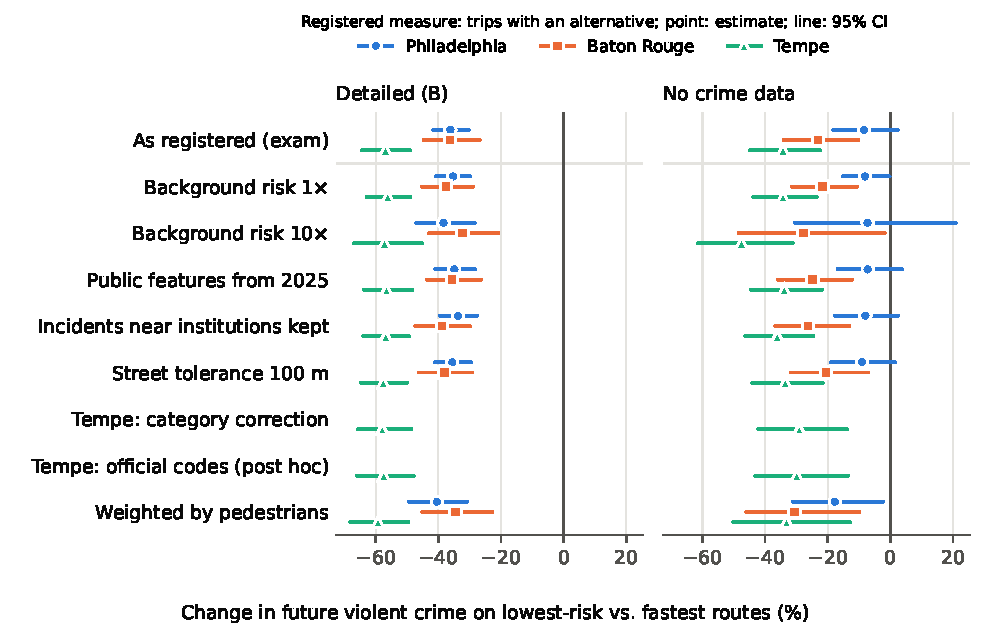
\includegraphics[width=\textwidth]{figuras/fig_sensibilidad.pdf}
\caption{Sensitivity analyses after the exam (exploratory). Registered measure for Detailed (B) and No crime data under each variant; the first row repeats the registered exam result. Points are estimates and lines 95\% intervals. The numbers are in Table~\ref{tab:sensibilidad}; its last row, which changes only the interval, is not plotted.}
\label{fig:sensibilidad}
\end{figure}

\paragraph{Router quality} Using the Lagrangian bound of the constrained problem \citep{handler1980dual}, we checked how close the route a pedestrian would take (the lowest-risk route when offered, otherwise the fastest) came to the lowest predicted exposure achievable within the same time limit. Over 2,000 trips per city and two maps, the median gap was 0.01--0.35 percentage points of the fastest route's predicted exposure, and the gap was at most 3 points in 98.7--100\% of trips (\ref{app:sensibilidad}, Table~\ref{tab:buscador}). In 0--1.2\% of trips, a route with at least 3 points less predicted exposure existed within the limit but was not offered. The gap concerns predicted exposure, the quantity the router optimizes, not future crime.

\paragraph{Background risk} The background term, three times the city's mean risk in the exam, penalizes length. With one and ten times the mean, the registered change of Detailed (B) stayed between $-32\%$ and $-38\%$ in Philadelphia and Baton Rouge and at $-56\%$ to $-57\%$ in Tempe (Table~\ref{tab:sensibilidad}). The term mainly controls how often an alternative is offered and how long the detour is. At $1\times$, alternatives were offered on 63--81\% of trips, with median detours of 1.3--2.2 minutes, and the change over all trips was $-31\%$ to $-52\%$. At $10\times$, they were offered on 13--29\% of trips, with median detours of 0.3--0.6 minutes, and the change over all trips was $-12\%$ to $-25\%$. Like the detour limit, the background term is a service setting that trades coverage for detour length. The No-crime-data level ranged from $-7\%$ to $-8\%$ in Philadelphia, $-22\%$ to $-28\%$ in Baton Rouge and $-34\%$ to $-48\%$ in Tempe.

\paragraph{Model versus a map of past crime} On all trips and on the same trips, we compared each model with the heat map built from the same past crime information (paired differences, 95\% intervals resampling 1-km zones). With the information of Detailed (B), the model and the heat map did not differ clearly in any city: $+1.7$ percentage points in Philadelphia ($-2.2$ to $+5.3$), $-4.4$ in Baton Rouge ($-9.7$ to $+0.8$) and $+1.2$ in Tempe ($-4.4$ to $+7.8$). With core crime only (A), the model avoided clearly more crime only in Tempe, the city with the fewest core incidents: $-15.4$ points ($-22.6$ to $-7.7$), against $-0.2$ in Philadelphia and $-3.6$ in Baton Rouge, whose intervals included zero. The registered test, on the trips where both maps offered an alternative, had also found it superior in Baton Rouge, by a small margin (Table~\ref{tab:hipotesis}). With street-level data, then, a simple map of past crime captures most of what the model offers; the model may help where the city's own records are sparse.

\paragraph{Per-person measure} The registered per-person measure divides each segment's crimes by its simulated pedestrians, with a floor at the median volume of segments with pedestrians. It proved sensitive to that floor (\ref{app:sensibilidad}, Table~\ref{tab:r7}). With the floor at the 75th percentile, every crime-by-street level reduced per-person risk in every city ($-27\%$ to $-46\%$). With the floor at the 25th percentile, 7 of the 9 city--level combinations increased it. Restricted to the day bands, where simulated volumes are better supported, the changes ranged from $-27\%$ to $+27\%$. The registered per-person results should therefore be read as indicative only.

\paragraph{Trips weighted by pedestrians} Random trips give equal weight to quiet and busy areas. When each trip was weighted by the simulated pedestrian volume along its fastest route, the registered change of the crime-by-street levels was $-35\%$ to $-46\%$ in Philadelphia, $-27\%$ to $-35\%$ in Baton Rouge and $-48\%$ to $-59\%$ in Tempe, with all intervals below zero. The No-crime-data level changed by $-18\%$ in Philadelphia (95\% CI $-31$ to $-2$), $-31\%$ in Baton Rouge and $-33\%$ in Tempe.

\paragraph{Two further versions of G16} We ran G16 with its single-bandwidth kernel, as written in the paper, and with a density restricted to the crimes of the trip's time band, which gives it the time information our models use; \citet{galbrun2014safe} propose such filtering but did not use it in their experiments. Neither changed the comparison (\ref{app:sensibilidad}, Table~\ref{tab:g16variantes}). With sums over vertices, G16 still increased crime on routes in Philadelphia ($+21\%$ to $+25\%$ over all trips); with uniform sampling, it reduced crime by 3--15\%. Our models avoided more future crime than each version in every city: all 24 paired 95\% intervals were below zero. Scott's rule gave kernels with a standard deviation of about 800--1,070 m with core crime and 470--720 m with all crime, and up to about 1,500 m when restricted to one time band.

\paragraph{Overdispersed crime counts} The stricter interval of Section~\ref{sec:robustness} redraws each future count from a Poisson distribution. To check whether crime clusters in time beyond that, we split each segment's future core incidents into the two halves of the scored year. Their dispersion relative to a binomial split was 1.08 in Philadelphia, 1.12 in Baton Rouge and 1.08 in Tempe, close to the value of 1 expected without clustering. Redrawing counts from a negative binomial distribution with that dispersion barely changed the intervals (Table~\ref{tab:sensibilidad}, last row). All three crime-by-street levels remained below zero in every city, for example from $-46\%$ to $-25\%$ for Detailed (B) in Philadelphia and from $-71\%$ to $-37\%$ in Tempe. The No-crime-data level remained below zero only in Tempe.

\paragraph{Tempe's crime categories} Tempe's categories were translated with generic keyword rules written before its data were opened. After the exam, an audit of every description found that most of them begin with a bracketed code that matches the official NIBRS code. The rules counted 1,932 records in the study period as core violent crime, before the exclusions of Section~\ref{sec:data}; according to the official code, 451 of them are not core: 218 cases of aggravated DUI [90D], 202 assaults that Arizona law calls aggravated but NIBRS classifies as simple [13B], and 31 cases of criminal damage [290]. Another 15 records counted as core carry no official code. The rules also missed 88 core records, including 18 homicides: the word ``non-negligent'' triggered the rule that excludes negligent killings. Two re-scorings left Tempe's results for the crime-by-street levels essentially unchanged (Table~\ref{tab:sensibilidad}). The first, specified in the plan before the audit, recodes the 249 records of aggravated DUI and criminal damage; Detailed (B) then changed future core crime by $-58\%$, against $-57\%$ in the exam. The second, decided after viewing the descriptions and therefore reported as post hoc, uses the official code wherever there is one; it changed the core records before exclusions from 1,932 to 1,569 (Table~\ref{tab:datos} counts 1,736 after exclusions with the registered rules), and Detailed (B) changed future core crime by $-57\%$, Coarse (C) by $-61\%$ and No crime data by $-30\%$ (exam: $-57\%$, $-52\%$ and $-34\%$).

\paragraph{Public features from before the scored period} The registered public features used OpenStreetMap data and transit schedules from 2026, which describe the cities during the scored period. We rebuilt every feature derived from them with the OpenStreetMap snapshot of 1 January 2025 \citep{osm_geofabrik} and with the transit schedules that SEPTA published on 30 August 2025 for Philadelphia \citep{septa_gtfs}. No earlier schedules could be found for Baton Rouge or Tempe, so their 2026 schedules were kept. The walking network and the Census, jobs and night-light data were unchanged, and the sealed models were applied again. Two checks preceded the analysis: from a practice city's original inputs, the rebuilding program reproduced all 37 model features exactly, and with the original features it reproduced the 27 exam maps of the three cities. With the 2025 features, the registered change of Detailed (B) was $-35\%$ in Philadelphia, $-36\%$ in Baton Rouge and $-57\%$ in Tempe (exam: $-36\%$, $-36\%$ and $-57\%$). Every level stayed within 3 percentage points of its exam value (\ref{app:sensibilidad}, Table~\ref{tab:r3}); the largest change, among the simple rules, was ``avoid commercial areas'' in Philadelphia ($-6\%$, against $-12\%$).

\paragraph{Exclusion rules} We relaxed the two exclusions that remove incidents with a valid location from the data. Keeping the incidents within 30 m of prisons, hospitals, police stations and social facilities added 78--930 core incidents per city over the study period. Raising the tolerance for the distance to a walkable street from 50 m to 100 m added 59--190. Both changes alter the past crime features and the future outcomes. The registered change of Detailed (B) was $-34\%$ and $-36\%$ in Philadelphia, $-39\%$ and $-38\%$ in Baton Rouge, and $-57\%$ and $-58\%$ in Tempe (exam: $-36\%$, $-36\%$ and $-57\%$). No crime data gave $-8\%$ and $-9\%$ in Philadelphia, $-26\%$ and $-21\%$ in Baton Rouge, and $-36\%$ and $-34\%$ in Tempe. With the exam's rules, the rebuilding program reproduced each city's exam crime map, with a maximum difference below $10^{-13}$.

% =========================================================================
\section{Deviations from the registered plan}\label{sec:deviations}
We report every deviation; details and dates are in the registrations' attachments.

\paragraph{Tempe's first download was stale} The vault had downloaded Tempe through a pregenerated ArcGIS Hub export that ended on 29 June 2024. The live service held records through October 2026. Tempe therefore had no scored-period data, and the oracle's flat map exposed the problem; Tempe was declared not evaluable. Because no Tempe result for the scored period had ever existed, we pre-registered a replacement exam \citep{osf_tempe}:
\begin{itemize}
  \item a direct download from the official service, sealed only after blind checks of period coverage and completeness;
  \item a corrected reading of Tempe's timestamps, which are local time labeled as UTC;
  \item a reading check that requires data in every study month.
\end{itemize}
The models were unchanged. The three-city results in Table~\ref{tab:hipotesis} are therefore an assessment completed with a replacement download, not the original confirmatory test.

\paragraph{Code fix} The exam program stopped when a map produced no lowest-risk route (Tempe's flat oracle). It was fixed to record such results as not available, as the plan already prescribed. The rerun of Philadelphia and Baton Rouge recomputed their maps, quick captures, paired comparisons and traps from the opened data, reusing their saved routes; its six score files were byte-identical to those of the first run.

\paragraph{Clarified trap rule} A dry run on synthetic data showed that the trap rule (``closer to chance than to the real map'') can flag a perfect trap when the real map is itself at chance level. Before the Tempe exam, the rule was clarified for that case; it gives identical verdicts whenever the real map beats chance, as in all traps reported here.

\paragraph{Documentation} The main registration misstated the random seed of the route-change intervals; the sealed code used seed 1.

\paragraph{Temporal leakage in public features} OpenStreetMap was downloaded in October 2026 and the transit schedules were those in force in 2026, so both describe the city during the scored period. This is information about the city, not about crime, and it affects all levels alike; it should nevertheless be removed in future versions. Rebuilding these features from data that predate the scored period changed every level by at most 3 percentage points (Section~\ref{sec:sensitivity}).

% =========================================================================
\section{Discussion}\label{sec:discussion}

\paragraph{What the results show} How much a crime-aware router can avoid depends mainly on the crime information a city provides, not on the sophistication of the predictor. With street-level records, routes chosen with a model trained in other cities avoided a large share of the city's \emph{future} recorded violent crime at a cost of about a minute. This held in three cities of different size and form, under a protocol designed to prevent leakage. Coarse categories performed about as well as detailed ones, and a simple map of the city's own past crime performed about as well as the model (Section~\ref{sec:sensitivity}), as in long-term crime forecasting at micro places \citep{wheeler2021rtm}. With core crime only, the model was superior to the map in the registered test in Baton Rouge and Tempe, but over all trips the difference was clear only in Tempe, the city with the sparsest records. At the aggregated levels, where no street-level map can be drawn, the model retained 45--64\% of the benefit, but it retained nearly as much without any crime data (44--59\%): zone counts and city-wide totals added little to public data alone. We did not test simpler ways of using aggregated data. With aggregates or public data alone, then, the benefit roughly halved and became comparable to that of a simple rule.

\paragraph{Robustness} The registered result held in the exploratory analyses after the exam. The router came within a fraction of a percentage point of the lowest predicted exposure achievable within the time limit. The reduction obtained with Detailed (B) changed little with the background risk, with public features rebuilt from data that predate the scored period, with other exclusion rules, with Tempe's crime categories corrected, with trips weighted by pedestrian volume and with overdispersed crime counts (Table~\ref{tab:sensibilidad}). The per-person measure, by contrast, depended on how sparsely walked streets are handled and should be read as indicative only.

\paragraph{Implications for pedestrian navigation services} The data-availability levels map onto deployment decisions.
\begin{itemize}
  \item \textbf{What a city needs to publish.} A city that releases incident locations with broad categories (violent, property, other) supports routes about as useful as one that releases detailed records, and a service can then build its risk map directly from the city's past crime. Aggregates by zone or city-wide totals retained 45--64\% of the benefit, little more than public data alone; the release that matters is that of incident locations.
  \item \textbf{What a service can offer without crime data.} Without the city's own records, a service should be cautious in presenting its routes as safer: the change ranged from $-8\%$ to $-34\%$ across cities and was not shown to beat a simple ``avoid commercial areas'' rule.
  \item \textbf{How long a detour to propose.} With street-level data, a 2-minute limit kept most of the benefit and a 5-minute limit nearly all of it. A service can therefore keep detours short at little loss. Without crime data, longer detours did not help.
  \item \textbf{How to read the city's categories.} Official offense codes should be used when a city publishes them. In Tempe, generic keyword rules misclassified nearly a quarter (23\%) of the records they counted as core violent crime, although the route results changed little once corrected.
  \item \textbf{Operation.} On a laptop and without any speed-up technique, the median query took under a second and 95\% of queries under 2 seconds. If every pedestrian followed the suggestions, walking would be spread across streets almost as it is on the fastest routes.
\end{itemize}

\paragraph{What they do not show} With aggregated data or no crime data at all, the model kept only about half of the benefit of street-level data, and without crime data it was never shown to beat a simple ``avoid commercial areas'' rule. With OpenStreetMap features alone (Map only), the result was even less reliable: it had no effect in Baton Rouge. The original motivation, giving data-poor cities routes as safe as data-rich ones, is therefore not yet achieved. This is the target of the next version, which will be tested on the still-closed reserve cities.

\paragraph{Limitations}
\begin{enumerate}
  \item \textbf{Exposure, not victimization.} We measure exposure to \emph{recorded} violent crime on route segments, not victimization; police records reflect reporting and enforcement \citep{lum2016predict}. We do not address road-traffic safety, which a pedestrian navigation service must also consider.
  \item \textbf{Two denominators.} The registered metric is computed over trips where the router offers an alternative. The all-trips effect is smaller, and we report both.
  \item \textbf{Trips and walking behavior.} Trips are drawn at random rather than from observed demand; weighting them by simulated pedestrian volumes did not change the result. Every pedestrian walks at 80 m/min without waiting at crossings, and four hours stand for the four time bands. The transport analyses assume that every pedestrian follows the suggestion.
  \item \textbf{Simulated data levels.} The data-availability levels were simulated by withholding information in cities that publish detailed data. A city that truly publishes less may differ in other ways.
  \item \textbf{Training period.} The models were trained on outcomes from the same period in which they were evaluated, although in other cities. A deployed system would train on an earlier period.
  \item \textbf{Scope.} Three U.S. exam cities are a small and specific sample.
  \item \textbf{Tempe's categories.} The generic keyword rules registered for Tempe misclassified nearly a quarter (23\%) of the records they counted as core violent crime and missed 88 core records (Section~\ref{sec:sensitivity}). Corrected re-scorings left the results for the crime-by-street levels essentially unchanged, but the registered Tempe outcome includes those errors.
  \item \textbf{Temporal leakage.} The registered features used OpenStreetMap data and transit schedules from 2026. Rebuilding them from data that predate the scored period changed every level by at most 3 percentage points (Section~\ref{sec:sensitivity}), but the walking network itself, and the schedules of Baton Rouge and Tempe, could not be replaced by earlier versions.
  \item \textbf{Simulated pedestrians.} The per-person metric depends on simulated volumes and on the floor applied to sparsely walked segments, and no night-time counts were available to validate the night bands.
\end{enumerate}

\paragraph{Ethics} The model uses no demographic or poverty variables, and its outputs are route choices, not area labels. Routing many pedestrians away from some streets could affect those streets' businesses and residents; this deserves study before large-scale deployment.

% =========================================================================
\section{Conclusions}
How much crime information does crime-aware pedestrian routing need? In a pre-registered, out-of-city evaluation, street-level incident locations, even with only broad categories, were enough for routes that avoid much of a city's future recorded violent crime at a cost of about a minute. With such data, a simple map of past crime did about as well as a transferred model. Aggregated data added little to public data alone: with them, or with national public data but no crime data, routes kept about half of the benefit, comparable to a simple rule; with OpenStreetMap alone, the result ranged from no effect to a large reduction. In exploratory analyses, the result was robust, a detour limit of two minutes kept most of the benefit, and the median routing query took under a second on a laptop. For pedestrian navigation services, the limiting factor is the city's crime data, not the detour, the computation or the predictor.

\FloatBarrier
\section*{Data and code availability}
\paragraph{Data} Police incident data are public and come from each city's open-data portal:
\begin{itemize}
  \item Philadelphia (exam): OpenDataPhilly, \texttt{incidents\_part1\_part2};
  \item Baton Rouge (exam): data.brla.gov, dataset \texttt{pbin-pcm7};
  \item Tempe (exam): City of Tempe, ``General Offenses (Open Data)'';
  \item Pittsburgh (learning): Pittsburgh Bureau of Police incident data, Western Pennsylvania Regional Data Center;
  \item Chapel Hill (learning): ArcGIS service \texttt{Recoded\_Incidents\_New} of the town's open-data portal;
  \item Chicago (learning): data.cityofchicago.org, dataset \texttt{ijzp-q8t2};
  \item Seattle (learning): data.seattle.gov, dataset \texttt{tazs-3rd5};
  \item Cincinnati (practice): data.cincinnati-oh.gov, datasets \texttt{8xzn-kpn7} and \texttt{7aqy-xrv9};
  \item Gainesville (practice): data.cityofgainesville.org, dataset \texttt{gvua-xt9q}.
\end{itemize}
Public features come from OpenStreetMap (Geofabrik extracts), the 2020 U.S. Census, LEHD LODES 2023, the cities' GTFS feeds and NASA VIIRS night-time radiance.

\paragraph{Registrations} The two pre-registrations, with the sealed models, the seal fingerprints, the vault manifest and the protocol documents, are on OSF \citep{osf_main,osf_tempe}. They will be made public at submission.

\paragraph{Analysis plans} The plans of the exploratory analyses (Section~\ref{sec:exploratory}) were committed to the author's version-control repository before their code was written. Every committed version of each plan, with its commit identifier and time, is included in the code release below.

\paragraph{Results} The aggregated results (every table in this paper and the per-city route outcomes) are included in the code release below.

\paragraph{Code} The analysis code, the routing engine, the aggregated results and the study documents are openly available under the MIT license \citep{codigo_zenodo}.

\section*{CRediT authorship contribution statement}
\textbf{Sergio Alberto Yacolca Cueva:} Conceptualization, Methodology, Software, Formal analysis, Investigation, Data curation, Visualization, Writing -- original draft, Writing -- review \& editing.

\section*{Funding}
This research did not receive any specific grant from funding agencies in the public, commercial, or not-for-profit sectors.

\section*{Declaration of competing interest}
The author has developed a non-commercial prototype of a pedestrian routing application that uses methods described in this paper. The author has received no income or other compensation related to this work.

\section*{Declaration of generative AI and AI-assisted technologies in the manuscript preparation process}
During the preparation of this work the author used Claude (Anthropic) to help write code and text and to review drafts, and ChatGPT (OpenAI) to review drafts. After using these tools, the author reviewed and edited the content as needed and takes full responsibility for the content of the published article. The author directed the study design, held the only key to the holdout data and ran the exams.

\bibliographystyle{elsarticle-harv}
\bibliography{refs}

\appendix
% Tablas numeradas por apendice (A.1, A.2, B.1...); hyperref necesita nombres unicos
\counterwithin*{table}{section}
\renewcommand{\theHtable}{app.\thetable}
\section{Model features, settings and exclusions}\label{app:modelo}
Table~\ref{tab:exclusiones} gives the records excluded by reason in each exam city. Table~\ref{tab:rasgos} lists the features of each level, read from the code of the sealed models. Public features are the same in every level except Map only, which uses only OpenStreetMap features and takes transit stops from OpenStreetMap instead of the schedules. Crime features describe the \emph{past} period and are expressed relative to the city mean in each time band. The target of every model is the segment's future core risk, spread in the same way and also relative to the city mean. Settings are in Section~\ref{sec:methods}.

\begin{table}[H]
\centering\small
\caption{Exam records in the study period (January 2024 to August 2026) by reason for exclusion. Institutions are prisons, hospitals, police stations and social facilities mapped in OpenStreetMap.}
\label{tab:exclusiones}
\ajustar{\begin{tabular}{lrrr}
\toprule
Reason & Philadelphia & Baton Rouge & Tempe \\
\midrule
Records in the study period & 413,305 & 67,021 & 76,143 \\
\midrule
No valid location & 10,736 (2.6\%) & 7,497 (11.2\%) & 183 (0.2\%) \\
No valid date & 0 (0.0\%) & 0 (0.0\%) & 670 (0.9\%) \\
Sexual offense & 4,425 (1.1\%) & 749 (1.1\%) & 1,107 (1.5\%) \\
Outside the city & 63 (0.0\%) & 233 (0.3\%) & 574 (0.8\%) \\
More than 50 m from a walkable street & 6,239 (1.5\%) & 3,462 (5.2\%) & 3,626 (4.8\%) \\
Within 30 m of an institution & 9,788 (2.4\%) & 701 (1.0\%) & 1,304 (1.7\%) \\
\midrule
Kept & 382,054 (92.4\%) & 54,379 (81.1\%) & 68,679 (90.2\%) \\
\bottomrule
\end{tabular}
}
\end{table}

\begin{table}[p]
\centering\scriptsize
\caption{Features by data-availability level (B = Detailed, A = Core only, C = Coarse, Total = City total, None = No crime data, Map = Map only). Distances are measured from the midpoint of the segment.}
\label{tab:rasgos}
\begin{tabular}{p{0.52\textwidth}ccccccc}
\toprule
Feature & B & A & C & Zone & Total & None & Map \\
\midrule
Segment length & $\bullet$ & $\bullet$ & $\bullet$ & $\bullet$ & $\bullet$ & $\bullet$ & $\bullet$ \\
Segment type (OpenStreetMap highway class; categorical) & $\bullet$ & $\bullet$ & $\bullet$ & $\bullet$ & $\bullet$ & $\bullet$ & $\bullet$ \\
Footpath away from streets (0/1) & $\bullet$ & $\bullet$ & $\bullet$ & $\bullet$ & $\bullet$ & $\bullet$ & $\bullet$ \\
Inside a park (0/1) & $\bullet$ & $\bullet$ & $\bullet$ & $\bullet$ & $\bullet$ & $\bullet$ & $\bullet$ \\
Distance to the nearest trunk, primary or secondary road & $\bullet$ & $\bullet$ & $\bullet$ & $\bullet$ & $\bullet$ & $\bullet$ & $\bullet$ \\
Shops and selected amenities within 150 m & $\bullet$ & $\bullet$ & $\bullet$ & $\bullet$ & $\bullet$ & $\bullet$ & $\bullet$ \\
Shops and selected amenities within 400 m & $\bullet$ & $\bullet$ & $\bullet$ & $\bullet$ & $\bullet$ & $\bullet$ & $\bullet$ \\
Street intersections (3+ streets) within 300 m & $\bullet$ & $\bullet$ & $\bullet$ & $\bullet$ & $\bullet$ & $\bullet$ & $\bullet$ \\
Intersections reachable along streets within 400 m & $\bullet$ & $\bullet$ & $\bullet$ & $\bullet$ & $\bullet$ & $\bullet$ & $\bullet$ \\
Schools within 400 m & $\bullet$ & $\bullet$ & $\bullet$ & $\bullet$ & $\bullet$ & $\bullet$ & $\bullet$ \\
Universities and colleges within 400 m & $\bullet$ & $\bullet$ & $\bullet$ & $\bullet$ & $\bullet$ & $\bullet$ & $\bullet$ \\
Hospitals within 400 m & $\bullet$ & $\bullet$ & $\bullet$ & $\bullet$ & $\bullet$ & $\bullet$ & $\bullet$ \\
Police stations within 800 m & $\bullet$ & $\bullet$ & $\bullet$ & $\bullet$ & $\bullet$ & $\bullet$ & $\bullet$ \\
Fuel stations within 150 m & $\bullet$ & $\bullet$ & $\bullet$ & $\bullet$ & $\bullet$ & $\bullet$ & $\bullet$ \\
Rail and transit stations within 400 m & $\bullet$ & $\bullet$ & $\bullet$ & $\bullet$ & $\bullet$ & $\bullet$ & $\bullet$ \\
Stadiums within 800 m & $\bullet$ & $\bullet$ & $\bullet$ & $\bullet$ & $\bullet$ & $\bullet$ & $\bullet$ \\
Shops and amenities open within 150 m (by band, opening hours) & $\bullet$ & $\bullet$ & $\bullet$ & $\bullet$ & $\bullet$ & $\bullet$ & $\bullet$ \\
Bars, pubs and nightclubs open within 150 m (by band) & $\bullet$ & $\bullet$ & $\bullet$ & $\bullet$ & $\bullet$ & $\bullet$ & $\bullet$ \\
Transit stops mapped in OpenStreetMap within 300 m &  &  &  &  &  &  & $\bullet$ \\
Residents within 400 m (Census 2020) & $\bullet$ & $\bullet$ & $\bullet$ & $\bullet$ & $\bullet$ & $\bullet$ &  \\
Jobs within 400 m (LODES 2023) & $\bullet$ & $\bullet$ & $\bullet$ & $\bullet$ & $\bullet$ & $\bullet$ &  \\
Night-time radiance (VIIRS) & $\bullet$ & $\bullet$ & $\bullet$ & $\bullet$ & $\bullet$ & $\bullet$ &  \\
Scheduled transit stops within 300 m (GTFS) & $\bullet$ & $\bullet$ & $\bullet$ & $\bullet$ & $\bullet$ & $\bullet$ &  \\
Bus departures per hour within 150 m (by band, typical Wednesday) & $\bullet$ & $\bullet$ & $\bullet$ & $\bullet$ & $\bullet$ & $\bullet$ &  \\
Simulated pedestrians per hour (by band) & $\bullet$ & $\bullet$ & $\bullet$ & $\bullet$ & $\bullet$ & $\bullet$ &  \\
Time band (categorical) & $\bullet$ & $\bullet$ & $\bullet$ & $\bullet$ & $\bullet$ & $\bullet$ & $\bullet$ \\
\midrule
Core incidents, spread (by band) & $\bullet$ & $\bullet$ &  &  &  &  &  \\
Core incidents, spread (all bands) & $\bullet$ & $\bullet$ &  &  &  &  &  \\
All incidents of the broad definition, spread (by band) & $\bullet$ &  &  &  &  &  &  \\
The same, all bands & $\bullet$ &  &  &  &  &  &  \\
Each of the ten broad categories, spread (all hours; 10 features) & $\bullet$ &  &  &  &  &  &  \\
Incidents in each bag (violent, property, other), spread, by band and all bands (6 features) &  &  & $\bullet$ &  &  &  &  \\
Core incidents per km of street in the Census block group (by band) & $\bullet$ & $\bullet$ &  & $\bullet$ &  &  &  \\
The same, all bands & $\bullet$ & $\bullet$ &  & $\bullet$ &  &  &  \\
City-wide core incidents per year per 1,000 residents & $\bullet$ & $\bullet$ & $\bullet$ & $\bullet$ & $\bullet$ &  &  \\
\bottomrule
\end{tabular}

\end{table}

\section{Quick capture}\label{app:rapida}
Table~\ref{tab:rapida} gives the quick capture of every map: the share of future core incidents that falls in the 10\% of network length that the map ranks as riskiest, averaged over the four time bands. A map without information captures about 0.10, and the oracle is the ceiling. It is a registered secondary metric; the trap rules of Section~\ref{sec:methods} use it.

\begin{table}[H]
\centering\small
\caption{Quick capture: share of future core incidents in the riskiest 10\% of network length (95\% CI, resampling 1-km zones). Chance is about 0.10.}
\label{tab:rapida}
\ajustar{\begin{tabular}{lccc}
\toprule
Map & Philadelphia & Baton Rouge & Tempe \\
\midrule
Detailed (B) & 0.43 (0.40, 0.45) & 0.47 (0.43, 0.50) & 0.58 (0.53, 0.63) \\
Core only (A) & 0.40 (0.37, 0.43) & 0.46 (0.42, 0.49) & 0.53 (0.48, 0.58) \\
Coarse (C) & 0.42 (0.39, 0.45) & 0.47 (0.43, 0.51) & 0.59 (0.54, 0.64) \\
Zone & 0.32 (0.30, 0.35) & 0.29 (0.25, 0.33) & 0.42 (0.35, 0.47) \\
City total & 0.19 (0.16, 0.21) & 0.19 (0.16, 0.23) & 0.36 (0.30, 0.42) \\
No crime data & 0.17 (0.15, 0.20) & 0.19 (0.16, 0.24) & 0.35 (0.29, 0.44) \\
Map only & 0.16 (0.13, 0.19) & 0.17 (0.14, 0.20) & 0.35 (0.28, 0.41) \\
Heat map B (no model) & 0.41 (0.39, 0.44) & 0.44 (0.40, 0.47) & 0.57 (0.51, 0.63) \\
Heat map A (no model) & 0.37 (0.35, 0.40) & 0.38 (0.34, 0.41) & 0.44 (0.38, 0.50) \\
Rule: avoid commercial areas & 0.14 (0.10, 0.17) & 0.11 (0.08, 0.14) & 0.25 (0.16, 0.33) \\
Rule: avoid arterials & 0.12 (0.10, 0.14) & 0.08 (0.06, 0.10) & 0.31 (0.25, 0.38) \\
Oracle (future crime; ceiling) & 0.84 (0.81, 0.86) & 1.00 (1.00, 1.00) & 1.00 (1.00, 1.00) \\
\bottomrule
\end{tabular}
}
\end{table}

\FloatBarrier
\section{Simulated pedestrian volumes}\label{app:peatones}
\paragraph{Model} People walk between places, so we simulate a weekday of walking trips over the street network and count how many pass along each segment in each time band. Origins and destinations are:
\begin{itemize}
  \item residents (Census blocks): trips to shops and jobs;
  \item transit stops (GTFS): trips to residents, jobs and shops;
  \item parking lots (OpenStreetMap): trips to jobs and shops;
  \item jobs (LEHD): trips to shops.
\end{itemize}
Daily trip rates are assumptions informed by the 2017 U.S. National Household Travel Survey, in which Americans made 3.37 trips per person per day, 10.5\% of them on foot, or about 0.35 walking trips per person per day \citep{mcguckin2018nhts}. Without ridership data, each scheduled bus departure counts as one boarding or alighting. A trip goes to a destination with probability proportional to the destination's weight times $\exp(-d/800\,\mathrm{m})$, where $d$ is the walking distance, and no trip is longer than 2,400 m. Trips follow shortest walking paths, and return trips are not counted because they use the same streets. Time-of-day profiles split trips into the four time bands; stops and shops use their own schedules. For large cities the simulation runs on 2-km tiles with a 2.4-km border, which gives the same result as the whole-city simulation.

\paragraph{Validation} We tested the model in New York City without tuning it to the city. The benchmark was 98 count locations of the NYC Department of Transportation \citep{nycdot_counts} (weekdays, 7--9 a.m. and 4--7 p.m., May 2023 to May 2026; bridges and the Hudson River greenway excluded, because walking there is mostly recreational). Spearman correlations between simulated and counted pedestrians, with 95\% bootstrap intervals, were:
\begin{itemize}
  \item \textbf{schedule-based transit} (the variant used in this paper): 0.56 (0.40 to 0.70);
  \item \textbf{observed subway ridership:} 0.67 (0.52 to 0.78);
  \item \textbf{an earlier heuristic} (buses per hour plus three times open shops): 0.41;
  \item \textbf{a direct-demand regression} \citep{schneider2009ped} fitted to the same city's counts and evaluated leaving each location out: 0.81 (0.71 to 0.87).
\end{itemize}
The simulation was most useful where the street network decides where people walk. In Manhattan, the ridership variant reached 0.67, against 0.14 for a direct-demand model fitted on the other boroughs. That variant produced about half of the counted volumes (median ratio 0.51), so simulated volumes are best read as relative.

\paragraph{Limitations} No night-time counts were available, so the night bands are not validated. The model has no tourism, recreational walking or campus trips.

\FloatBarrier
\section{Details of the exploratory analyses}\label{app:sensibilidad}
This appendix gives the tables of Section~\ref{sec:exploratory} that are not shown in the text:
\begin{itemize}
  \item the robustness checks of the registered measure (Table~\ref{tab:robustez});
  \item the cost of each detour budget, the concentration of walking and the time per routing query (Tables~\ref{tab:curvacosto}, \ref{tab:sistema} and~\ref{tab:tiempos});
  \item the quality of the router (Table~\ref{tab:buscador});
  \item two further versions of G16 (Table~\ref{tab:g16variantes});
  \item the public features rebuilt from data that predate the scored period (Table~\ref{tab:r3});
  \item the per-person measure with other floors for sparsely walked segments (Table~\ref{tab:r7}).
\end{itemize}
The plans of these analyses and their recorded changes are openly available with the code \citep{codigo_zenodo}.

\begin{table}[H]
\centering\small
\caption{Robustness (exploratory). Registered estimate (trip bootstrap); intervals resampling 1-km origin zones, and resampling zones plus Poisson-redrawn crime counts; and the change over all trips (lowest-risk route when offered, fastest otherwise). \%.}
\label{tab:robustez}
\ajustar{\begin{tabular}{llcccc}
\toprule
Level & City & \begin{tabular}[b]{@{}c@{}}Change, trips with an \\ alternative (trip CI)\end{tabular} & \begin{tabular}[b]{@{}c@{}}CI, 1-km \\ zones\end{tabular} & \begin{tabular}[b]{@{}c@{}}CI, zones and \\ redrawn crimes\end{tabular} & \begin{tabular}[b]{@{}c@{}}Change, all \\ trips (zone CI)\end{tabular} \\
\midrule
Detailed (B) & Philadelphia & -36 (-42, -30) & (-42, -30) & (-45, -26) & -25 (-30, -20) \\
Detailed (B) & Baton Rouge & -36 (-45, -27) & (-45, -26) & (-51, -17) & -26 (-33, -18) \\
Detailed (B) & Tempe & -57 (-64, -49) & (-65, -47) & (-71, -38) & -45 (-53, -36) \\
\midrule
Core only (A) & Philadelphia & -35 (-41, -28) & (-40, -28) & (-44, -24) & -23 (-28, -18) \\
Core only (A) & Baton Rouge & -28 (-37, -18) & (-39, -16) & (-45, -7) & -19 (-27, -11) \\
Core only (A) & Tempe & -52 (-60, -43) & (-61, -41) & (-67, -33) & -41 (-49, -31) \\
\midrule
Coarse (C) & Philadelphia & -39 (-45, -33) & (-45, -33) & (-49, -29) & -27 (-32, -22) \\
Coarse (C) & Baton Rouge & -33 (-42, -24) & (-43, -22) & (-51, -13) & -25 (-34, -16) \\
Coarse (C) & Tempe & -52 (-60, -43) & (-62, -40) & (-68, -30) & -44 (-54, -34) \\
\midrule
No crime data & Philadelphia & -8 (-18, +2) & (-19, +3) & (-24, +10) & -3 (-8, +1) \\
No crime data & Baton Rouge & -23 (-34, -10) & (-35, -8) & (-44, +5) & -11 (-18, -4) \\
No crime data & Tempe & -34 (-45, -22) & (-45, -21) & (-55, -10) & -22 (-30, -12) \\
\bottomrule
\end{tabular}
}
\end{table}

\begin{table}[H]
\centering\small
\caption{Cost of each detour budget: share of trips for which the router offered a lowest-risk route (Alt.), and median extra walking time of those routes in minutes (Extra min.).}
\label{tab:curvacosto}
\ajustar{\begin{tabular}{llrrrrrr}
\toprule
 & & \multicolumn{2}{c}{Philadelphia} & \multicolumn{2}{c}{Baton Rouge} & \multicolumn{2}{c}{Tempe} \\
Map & Detour limit & Alt. (\%) & Extra min. & Alt. (\%) & Extra min. & Alt. (\%) & Extra min. \\
\midrule
Detailed (B) & 2 min & 35\% & 0.4 & 41\% & 0.4 & 52\% & 0.5 \\
 & 5 min & 38\% & 0.6 & 46\% & 0.6 & 57\% & 0.8 \\
 & 10 min & 38\% & 0.6 & 48\% & 0.7 & 60\% & 1.0 \\
 & App default & 38\% & 0.6 & 48\% & 0.7 & 60\% & 1.1 \\
\midrule
No crime data & 2 min & 29\% & 0.4 & 26\% & 0.4 & 42\% & 0.4 \\
 & 5 min & 32\% & 0.5 & 31\% & 0.7 & 47\% & 0.7 \\
 & 10 min & 32\% & 0.5 & 33\% & 0.8 & 49\% & 0.7 \\
 & App default & 32\% & 0.5 & 33\% & 0.8 & 49\% & 0.8 \\
\midrule
Oracle (ceiling) & 2 min & 50\% & 0.6 & 35\% & 0.5 & 45\% & 0.6 \\
 & 5 min & 56\% & 1.0 & 43\% & 1.0 & 53\% & 1.2 \\
 & 10 min & 57\% & 1.1 & 46\% & 1.5 & 57\% & 2.3 \\
 & App default & 57\% & 1.1 & 47\% & 1.6 & 58\% & 2.6 \\
\bottomrule
\end{tabular}
}
\end{table}

\begin{table}[H]
\centering\small
\caption{Concentration of walking (descriptive) if every trip followed the fastest route or the app's suggestion (lowest-risk route when offered, otherwise the fastest), with the default limit, over the 2,000 random trips per city. Walked meters are counted per street segment.}
\label{tab:sistema}
\ajustar{\begin{tabular}{llrrrrrr}
\toprule
 & & \multicolumn{2}{c}{Distinct segments used} & \multicolumn{2}{c}{Meters on top 1\% segments} & \multicolumn{2}{c}{Gini of meters} \\
City & Map & Fastest & Suggested & Fastest & Suggested & Fastest & Suggested \\
\midrule
Philadelphia & Detailed (B) & 55,575 & 54,374 & 30.6\% & 31.3\% & 0.897 & 0.901 \\
 & No crime data & 55,575 & 55,243 & 30.6\% & 31.0\% & 0.897 & 0.899 \\
\midrule
Baton Rouge & Detailed (B) & 21,408 & 21,644 & 24.4\% & 25.2\% & 0.855 & 0.860 \\
 & No crime data & 21,408 & 21,869 & 24.4\% & 25.2\% & 0.855 & 0.857 \\
\midrule
Tempe & Detailed (B) & 28,411 & 29,225 & 29.6\% & 31.7\% & 0.882 & 0.885 \\
 & No crime data & 28,411 & 29,844 & 29.6\% & 31.6\% & 0.882 & 0.882 \\
\bottomrule
\end{tabular}
}
\end{table}

\begin{table}[H]
\centering\small
\caption{Time per routing query with the Detailed (B) map, first 200 trips per city, excluding network loading. One process on a laptop with an Intel Core i9-12900H processor and 32 GB of memory (Windows 11).}
\label{tab:tiempos}
\begin{tabular}{lrrrr}
\toprule
City & Street segments & Queries & Median (s) & 95th percentile (s) \\
\midrule
Philadelphia & 194,957 & 200 & 0.87 & 1.72 \\
Baton Rouge & 49,540 & 200 & 0.29 & 0.63 \\
Tempe & 70,028 & 200 & 0.50 & 1.08 \\
\bottomrule
\end{tabular}

\end{table}

\begin{table}[H]
\centering\small
\caption{Router quality (exploratory): gap between the predicted exposure of the route a pedestrian would take and the Lagrangian lower bound for any route within the same time limit, in percentage points of the fastest route's predicted exposure; 2,000 trips per city. Missed $\ge 3$: a route within the limit with at least 3 points less predicted exposure was not offered.}
\label{tab:buscador}
\ajustar{\begin{tabular}{llrrrrr}
\toprule
City & Map & Median gap & 95th pct. gap & Gap $\le 1$ & Gap $\le 3$ & Missed $\ge 3$ \\
\midrule
Philadelphia & Detailed (B) & 0.07 & 2.3 & 78.9\% & 99.8\% & 0.2\% \\
 & No crime data & 0.23 & 2.5 & 73.8\% & 100.0\% & 0.0\% \\
Baton Rouge & Detailed (B) & 0.01 & 2.5 & 79.5\% & 98.7\% & 1.2\% \\
 & No crime data & 0.10 & 2.3 & 78.8\% & 99.7\% & 0.3\% \\
Tempe & Detailed (B) & 0.13 & 2.5 & 75.5\% & 99.2\% & 0.5\% \\
 & No crime data & 0.35 & 2.5 & 68.8\% & 99.7\% & 0.4\% \\
\bottomrule
\end{tabular}
}
\end{table}

\begin{table}[H]
\centering\small
\caption{Two further versions of G16 (exploratory): change in future core incidents over all trips, \% (95\% CI resampling 1-km origin zones), followed by the paired difference with our model given the same information (Core only (A) for core crime, Detailed (B) for all crime), in percentage points; negative values mean that our model avoided more.}
\label{tab:g16variantes}
\ajustar{\begin{tabular}{lccc}
\toprule
G16 variant & Philadelphia & Baton Rouge & Tempe \\
\midrule
Isotropic kernel, core crime & +21 (+12, +30); -44 & +6 (-6, +19); -26 & +5 (-9, +20); -45 \\
Isotropic kernel, all crime & +23 (+14, +32); -48 & -1 (-11, +11); -26 & -4 (-16, +10); -40 \\
Isotropic, uniform sampling, core crime & -10 (-16, -4); -13 & -5 (-13, +3); -14 & -7 (-17, +4); -34 \\
Isotropic, uniform sampling, all crime & -5 (-11, +2); -20 & -6 (-12, +1); -20 & -15 (-25, -4); -29 \\
By time band, core crime & +25 (+16, +34); -48 & +9 (-3, +23); -29 & +1 (-13, +16); -41 \\
By time band, all crime & +22 (+14, +31); -48 & +3 (-8, +16); -30 & -0.4 (-15, +17); -44 \\
By time band, uniform sampling, core crime & -7 (-13, -2); -16 & -3 (-10, +5); -16 & -11 (-20, -2); -30 \\
By time band, uniform sampling, all crime & -8 (-14, +0); -17 & -6 (-12, +1); -20 & -15 (-24, -6); -30 \\
\bottomrule
\end{tabular}
}
\end{table}

\begin{table}[H]
\centering\small
\caption{Public features from before the scored period (exploratory): registered measure with features rebuilt from the OpenStreetMap snapshot of 1 January 2025 and, in Philadelphia, the transit schedules of 30 August 2025, \% (95\% CI); in brackets, the registered exam value.}
\label{tab:r3}
\ajustar{\begin{tabular}{lccc}
\toprule
Map & Philadelphia & Baton Rouge & Tempe \\
\midrule
Detailed (B) & -35 (-41, -28) [-36] & -36 (-44, -26) [-36] & -57 (-64, -48) [-57] \\
Core only (A) & -33 (-39, -27) [-35] & -29 (-38, -19) [-28] & -52 (-60, -43) [-52] \\
Coarse (C) & -39 (-45, -33) [-39] & -34 (-42, -24) [-33] & -51 (-59, -42) [-52] \\
Zone & -19 (-27, -11) [-17] & -20 (-31, -7) [-22] & -32 (-42, -20) [-35] \\
City total & -9 (-18, +2) [-11] & -20 (-33, -5) [-20] & -35 (-47, -23) [-35] \\
No crime data & -7 (-17, +4) [-8] & -25 (-36, -12) [-23] & -34 (-45, -22) [-34] \\
Map only & -8 (-18, +3) [-7] & +1 (-14, +19) [+4] & -42 (-52, -30) [-40] \\
Rule: avoid commercial areas & -6 (-18, +7) [-12] & -22 (-39, -4) [-20] & -30 (-44, -13) [-29] \\
Rule: avoid arterials & +12 (+1, +25) [+11] & +11 (-6, +32) [+13] & -37 (-49, -25) [-37] \\
\bottomrule
\end{tabular}
}
\end{table}

\begin{table}[H]
\centering\small
\caption{Per-person measure (registered secondary metric) with other floors for sparsely walked segments, and restricted to the day bands (6 a.m. to 6 p.m.), \% (95\% CI). Same trips and routes as the exam.}
\label{tab:r7}
\ajustar{\begin{tabular}{llccc}
\toprule
Map & Variant & Philadelphia & Baton Rouge & Tempe \\
\midrule
Detailed (B) & Median floor (registered) & -13 (-26, +1) & -29 (-46, -8) & -27 (-49, -0.3) \\
 & 25th-percentile floor & +8 (-10, +29) & -23 (-44, +7) & +25 (-24, +94) \\
 & 75th-percentile floor & -28 (-37, -18) & -42 (-56, -25) & -45 (-60, -29) \\
 & Day bands only & +2 (-13, +17) & +5 (-14, +29) & -27 (-54, +8) \\
\midrule
Core only (A) & Median floor (registered) & -10 (-23, +3) & -21 (-40, +4) & -28 (-49, -2) \\
 & 25th-percentile floor & +15 (-8, +39) & -6 (-33, +30) & +25 (-30, +103) \\
 & 75th-percentile floor & -28 (-37, -19) & -36 (-51, -17) & -44 (-58, -27) \\
 & Day bands only & +7 (-9, +24) & +27 (+4, +55) & -1 (-30, +33) \\
\midrule
Coarse (C) & Median floor (registered) & -10 (-23, +7) & -27 (-49, +3) & -16 (-43, +18) \\
 & 25th-percentile floor & +14 (-6, +39) & +23 (-21, +83) & +57 (-12, +148) \\
 & 75th-percentile floor & -27 (-36, -16) & -46 (-60, -27) & -43 (-59, -25) \\
 & Day bands only & -9 (-22, +6) & +9 (-12, +35) & +5 (-29, +52) \\
\midrule
Zone & Median floor (registered) & +9 (-7, +28) & -13 (-32, +12) & -17 (-39, +9) \\
 & 25th-percentile floor & +50 (+23, +86) & +15 (-21, +67) & +32 (-14, +97) \\
 & 75th-percentile floor & -10 (-22, +3) & -30 (-45, -12) & -39 (-53, -23) \\
 & Day bands only & +42 (+20, +66) & +27 (-3, +66) & +28 (-5, +73) \\
\midrule
City total & Median floor (registered) & +40 (+17, +67) & -39 (-54, -18) & -14 (-38, +16) \\
 & 25th-percentile floor & +110 (+69, +158) & -34 (-52, -7) & +20 (-29, +92) \\
 & 75th-percentile floor & +5 (-11, +22) & -42 (-54, -24) & -26 (-43, -4) \\
 & Day bands only & +49 (+25, +76) & +33 (-1, +81) & +40 (-3, +96) \\
\midrule
No crime data & Median floor (registered) & +47 (+23, +72) & -31 (-49, -9) & -6 (-32, +29) \\
 & 25th-percentile floor & +111 (+71, +159) & -10 (-40, +36) & +41 (-14, +129) \\
 & 75th-percentile floor & +13 (-3, +31) & -39 (-52, -24) & -22 (-40, +0.3) \\
 & Day bands only & +43 (+19, +72) & +19 (-10, +61) & +35 (-6, +94) \\
\midrule
Map only & Median floor (registered) & +11 (-10, +40) & +7 (-20, +46) & -31 (-51, -5) \\
 & 25th-percentile floor & +32 (-0.5, +78) & +29 (-20, +112) & -21 (-47, +18) \\
 & 75th-percentile floor & -4 (-19, +16) & -7 (-28, +19) & -41 (-57, -22) \\
 & Day bands only & +41 (+17, +71) & +39 (-3, +98) & +46 (+6, +99) \\
\bottomrule
\end{tabular}
}
\end{table}

\end{document}
